% ============================================================
%  Rapport Baligh+ — Réécriture de v2.pdf
%  Style : rapport_balligh_plus.tex / page_garde.tex
% ============================================================
\documentclass[12pt,a4paper]{report}

% ── Encodage & langue ──────────────────────────────────────
\usepackage[utf8]{inputenc}
\usepackage[T1]{fontenc}
\usepackage[francais]{babel}
\usepackage{iflang}
\usepackage{subcaption}
\usepackage{graphicx}

% ── Police Palatino (élégante & académique) ────────────────
\usepackage{palatino}
\usepackage{mathpazo}

% ── Mise en page ───────────────────────────────────────────
\usepackage[top=2.5cm,bottom=2.8cm,left=3cm,right=2.5cm,headheight=16pt]{geometry}
\usepackage{setspace}
\onehalfspacing

% ── Palette de couleurs ────────────────────────────────────
\usepackage{xcolor}
\definecolor{primary}{named}{NavyBlue}
\definecolor{accent}{named}{Goldenrod}
\definecolor{dark}{named}{MidnightBlue}
\definecolor{muted}{named}{Gray}
\definecolor{lightbg}{named}{LightGray}
\definecolor{rulecol}{named}{NavyBlue}
\definecolor{tabhead}{named}{DarkGray}
\definecolor{tabalt}{named}{Gray}

% ── Titres personnalisés ───────────────────────────────────
\usepackage{titlesec}
\titleformat{\chapter}[display]
  {\normalfont\Large\bfseries\color{primary}}
  {\textcolor{accent}{\chaptertitlename\ \thechapter}}{10pt}
  {\Huge\color{dark}}
  [\vspace{4pt}\textcolor{accent}{\titlerule[1.5pt]}]

\titleformat{\section}
  {\normalfont\large\bfseries\color{primary}}
  {\textcolor{accent}{\thesection}}{1em}{}
  [\vspace{-2pt}\textcolor{muted}{\titlerule[0.4pt]}]

\titleformat{\subsection}
  {\normalfont\normalsize\bfseries\color{dark}}
  {\textcolor{accent}{\thesubsection}}{1em}{}

% ── Tableaux ───────────────────────────────────────────────
\usepackage{booktabs}
\usepackage{tabularx}
\usepackage{longtable}
\usepackage{array}
\usepackage{multirow}
\usepackage{colortbl}
\usepackage{makecell}

% ── Listes ─────────────────────────────────────────────────
\usepackage{enumitem}
\setlist[itemize]{
  leftmargin=*,
  topsep=4pt,
  itemsep=2pt,
  label=\textcolor{accent}{\textbullet}
}
\setlist[enumerate]{
  leftmargin=*,
  topsep=4pt,
  itemsep=2pt,
  label=\textcolor{primary}{\arabic*.}
}

% ── Liens & PDF ────────────────────────────────────────────
\usepackage{hyperref}
\hypersetup{
  colorlinks=true,
  linkcolor=primary,
  urlcolor=accent,
  citecolor=muted,
  pdftitle={Baligh+ — Plateforme Intelligente de Signalement Urbain},
  pdfauthor={RAHAL Lyes, BAHAR Naceredine, BOUKHRISSA Yazid},
}

% ── En-têtes & pieds de page ───────────────────────────────
\usepackage{fancyhdr}
\pagestyle{fancy}
\fancyhf{}

\fancyhead[L]{%
  \small\textit{\textcolor{muted}{BALIGH+}}%
  \textcolor{accent}{\quad|\quad}%
}
\fancyhead[R]{%
  \small\textit{\textcolor{muted}{\leftmark}}%
}
\fancyfoot[C]{%
  \textcolor{accent}{\rule{1.5cm}{0.3pt}}\quad
  \textcolor{primary}{\thepage}%
  \quad\textcolor{accent}{\rule{1.5cm}{0.3pt}}%
}
\renewcommand{\headrulewidth}{0.4pt}
\renewcommand{\footrulewidth}{0pt}
\renewcommand{\headrule}{%
  {\color{primary}\hrule width\headwidth height 0.4pt}%
  \vspace{0.5pt}%
  {\color{accent}\hrule width 3cm height 0.8pt}%
}

% ── Divers ─────────────────────────────────────────────────
\usepackage{float}
\usepackage{amsmath}
\usepackage{amssymb}
\usepackage{wasysym}
\usepackage{microtype}
\usepackage{parskip}
\setlength{\parindent}{0pt}
\setlength{\parskip}{6pt}

% ── Macro utilitaire : cellule d'en-tête de tableau ────────
\newcommand{\thdcell}[1]{%
  \cellcolor{tabhead}\textbf{\textcolor{white}{#1}}%
}

% ── Support arabe (RTL) ────────────────────────────────────
\usepackage{arabtex}
\usepackage{utf8}
\setcode{utf8}

% ── Boîte de citation/note élégante ────────────────────────
\usepackage{tcolorbox}
\tcbuselibrary{skins}
\newtcolorbox{notebox}{
  enhanced,
  colback=lightbg,
  colframe=primary,
  boxrule=0.6pt,
  left=8pt, right=8pt, top=5pt, bottom=5pt,
  arc=2pt,
  fonttitle=\small\bfseries\color{primary},
}

% ============================================================
\begin{document}

% ── Page de garde ───────────────────────────────────────────
\begin{titlepage}

  \noindent
  \begin{minipage}[c]{0.15\linewidth}
    
\includegraphics[width=40pt]{./images/logo.png}
  \end{minipage}
  \hfill
  \begin{minipage}[c]{0.15\linewidth}
    \raggedleft
    
\includegraphics[width=40pt]{./images/logo.png}
  \end{minipage}

  \vspace{0.4cm}

  \begin{center}
    {\bfseries
      République Algérienne Démocratique et Populaire \\[0.2cm]
      Ministère de l'Enseignement Supérieur et de la Recherche Scientifique
    }

    \vspace{0.4cm}
    \rule{\linewidth}{1.5pt}\\[0.3cm]
    {\bfseries\large\textcolor{dark}{Université Akli Mohand Oulhadj de Bouira}} \\[0.2cm]
    {\bfseries Faculté des Sciences et des Sciences exactes} \\
    {\bfseries Département d'Informatique}\\[0.3cm]
    \rule{\linewidth}{1.5pt}

    \vspace{0.8cm}

    {\large\bfseries Mémoire de Master} \\[0.2cm]
    {\normalsize\bfseries en Informatique} \\[0.3cm]
    {\normalsize\emph{%
      \textbf{Spécialité :}
      Ingénierie des Systèmes d'Information et du Logiciel%
    }}

    \vspace{1cm}

    {\LARGE\bfseries\textcolor{dark}{Plateforme Intelligente de Signalement Urbain}}\\[0.6cm]
    {\large\textit{``\textbf{BALIGH+} Cas d'étude : commune de Bouira''}}

    \vspace{1.2cm}

    
\includegraphics[width=90pt]{./images/baligh_logo.png}

  \end{center}

  \begin{tabular}{p{0.45\linewidth} p{0.45\linewidth}}
    \textbf{Encadré par}       & \textbf{Réalisé par}   \\[6pt]
    \quad Mr DJOUABRI Abdrazak & \quad RAHAL Lyes       \\
                               & \quad BAHAR Naceredine \\
                               & \quad BOUKHRISSA Yazid \\
  \end{tabular}

  \vfill

  \begin{center}
    {\large\bfseries 2025/2026}
  \end{center}

\end{titlepage}

% ── Dédicace — RAHAL Lyes ───────────────────────────────────
\cleardoublepage
\thispagestyle{empty}
\vspace*{4cm}

\begin{center}
  {\large\textit{\textcolor{primary}{\bfseries Dédicace}}}\\[0.8cm]
  \rule{0.4\linewidth}{0.4pt}\\[1cm]

  {\normalsize\itshape
  Je dédie ce travail à mes chers parents, qui ont toujours été une source
  d'amour, de soutien et de motivation. Aucun mot ne saurait exprimer ma
  gratitude pour tous les sacrifices qu'ils ont consentis afin de me permettre
  de poursuivre mes études et de réaliser mes ambitions.

  À ma famille, pour son affection, sa confiance et ses encouragements tout au
  long de mon parcours.

  À mes amis et à toutes les personnes qui m'ont soutenu de près ou de loin.

  Enfin, à tous ceux qui croient en la valeur du savoir et de l'innovation.

  \vspace{1cm}
  \textit{« Le succès est la somme de petits efforts répétés jour après jour. »}

  }\\[1cm]

  \rule{0.4\linewidth}{0.4pt}\\[0.5cm]
  {\bfseries RAHAL Lyes}
\end{center}

\newpage

% ── Dédicace — BAHAR Naceredine ─────────────────────────────
\cleardoublepage
\thispagestyle{empty}
\vspace*{4cm}

\begin{center}
  {\large\textit{\textcolor{primary}{\bfseries Dédicace}}}\\[0.8cm]
  \rule{0.4\linewidth}{0.4pt}\\[1cm]

  {\normalsize\itshape
  Je dédie ce travail à mes parents, dont le soutien, la patience et les
  encouragements m'ont accompagné durant toutes ces années d'études.

  À mes frères, mes sœurs et toute ma famille pour leur présence et leur
  confiance.

  À mes enseignants qui ont contribué à ma formation et m'ont transmis des
  connaissances précieuses.

  À tous ceux qui m'ont aidé à avancer et à persévérer face aux difficultés.

  \vspace{1cm}
  \textit{« La persévérance transforme les rêves en réalité. »}

  }\\[1cm]

  \rule{0.4\linewidth}{0.4pt}\\[0.5cm]
  {\bfseries BAHAR Naceredine}
\end{center}

\newpage

% ── Dédicace — BOUKHRISSA Yazid ─────────────────────────────
\cleardoublepage
\thispagestyle{empty}
\vspace*{4cm}

\begin{center}
  {\large\textit{\textcolor{primary}{\bfseries Dédicace}}}\\[0.8cm]
  \rule{0.4\linewidth}{0.4pt}\\[1cm]

  {\normalsize\itshape
  Je dédie ce travail à mes très chers parents, pour leur amour, leurs sacrifices
  et leur soutien inconditionnel qui ont toujours éclairé mon chemin.

  À ma famille et à mes proches qui ont cru en moi et m'ont encouragé à donner
  le meilleur de moi-même.

  À mes camarades et amis avec qui j'ai partagé cette aventure universitaire.

  À toutes les personnes qui ont contribué à mon épanouissement personnel et
  professionnel.

  \vspace{1cm}
  \textit{« L'avenir appartient à ceux qui croient à la beauté de leurs rêves. »}

  }\\[1cm]

  \rule{0.4\linewidth}{0.4pt}\\[0.5cm]
  {\bfseries BOUKHRISSA Yazid}
\end{center}

\newpage

% ── Remerciements ───────────────────────────────────────────
\cleardoublepage
\thispagestyle{empty}
\chapter*{Remerciements}
\addcontentsline{toc}{chapter}{Remerciements}

Nous tenons tout d'abord à adresser nos sincères remerciements à notre
encadreur, \textbf{M. DJOUABRI Abdrazak}, pour sa disponibilité, ses précieux
conseils, son accompagnement rigoureux et son soutien tout au long de
l'élaboration de ce mémoire.

Nous remercions également l'ensemble du corps enseignant du \textbf{Département
  d'Informatique} de l'Université Akli Mohand Oulhadj de Bouira pour la qualité
de la formation dispensée au cours de nos années d'études et pour les
connaissances qui nous ont permis de mener à bien ce projet.

Nos remerciements s'adressent également à toute l'équipe de
l'\textbf{Incubateur de l'Université de Bouira}, et plus particulièrement aux
enseignants formateurs, pour leur encadrement, leurs conseils et leur
accompagnement dans le développement de notre esprit entrepreneurial et de nos
compétences en gestion de projet.

Nous exprimons également notre gratitude aux membres du jury pour l'intérêt
qu'ils portent à ce travail et pour le temps consacré à son évaluation.

Enfin, nous adressons notre profonde reconnaissance à nos familles, nos proches
et à toutes les personnes qui nous ont soutenus, de près ou de loin, par leurs
encouragements, leur confiance et leur soutien moral tout au long de notre
parcours universitaire. Sans leur appui, la réalisation de ce projet n'aurait
pas été possible.

\vspace{1cm}
\begin{flushright}
  \textit{RAHAL Lyes, BAHAR Naceredine, BOUKHRISSA Yazid}\\
  \textit{Bouira, 2025/2026}
\end{flushright}
\newpage

% ── Liste des abréviations ──────────────────────────────────
\cleardoublepage
\chapter*{Liste des Abréviations}
\addcontentsline{toc}{chapter}{Liste des Abréviations}

\begin{tabularx}{\linewidth}{>{\bfseries\color{primary}}lX}
  \toprule
  \rowcolor{primary}
  \textcolor{white}{\textbf{Abréviation}} &
  \textcolor{white}{\textbf{Signification}} \\
  \midrule

  API  & Application Programming Interface (Interface de Programmation Applicative) \\
  BD   & Base de Données \\
  CDD  & Cahier des Charges et Définition des besoins \\
  CSS  & Cascading Style Sheets (Feuilles de Style en Cascade) \\
  GPS  & Global Positioning System (Système de Positionnement Global) \\
  HTML & HyperText Markup Language \\
  HTTP & HyperText Transfer Protocol \\
  JS   & JavaScript \\
  MVC  & Modèle-Vue-Contrôleur \\
  MySQL & My Structured Query Language \\
  OSM  & OpenStreetMap \\
  PHP  & PHP : Hypertext Preprocessor \\
  RTL  & Right-To-Left (Écriture de droite à gauche) \\
  SI   & Système d'Information \\
  SQL  & Structured Query Language (Langage de Requête Structurée) \\
  UI   & User Interface (Interface Utilisateur) \\
  URL  & Uniform Resource Locator (Localisateur Uniforme de Ressource) \\
  UX   & User Experience (Expérience Utilisateur) \\
  WEBP & Web Picture Format \\

  \bottomrule
\end{tabularx}

% ── Liste des tableaux ──────────────────────────────────────
\listoftables
\addcontentsline{toc}{chapter}{Liste des Tableaux}
\newpage

% ── Liste des figures ───────────────────────────────────────
\listoffigures
\addcontentsline{toc}{chapter}{Liste des Figures}
\newpage

% ── Préface ─────────────────────────────────────────────────
\cleardoublepage
\chapter*{Préface}
\addcontentsline{toc}{chapter}{Préface}

\begin{flushright}
  {\small\textcolor{muted}{\textit{النسخة العربية}}}
\end{flushright}

\vspace{0.4cm}

\begin{RLtext}
  تشهد المدن الجزائرية اليوم تحوّلاتٍ عميقة تقودها أجيالٌ متّصلة بالعالم الرقمي، ودولةٌ تسعى إلى تحديث مختلف مرافقها وخدماتها. وفي خضمّ هذا التحوّل الشامل الذي يطال تدريجياً شتّى قطاعات الحياة العامة، تبقى إحدى الحلقات الأساسية بحاجة إلى مزيدٍ من التطوير، وهي العلاقة المباشرة بين المواطن والبلدية.

  في هذا السياق وُلد مشروع «بلّغ»، المستوحى اسمه من الفعل العربي «بلّغ» بمعنى الإخبار والإيصال. وهو منصّة رقمية ذكية تهدف إلى تسهيل الإبلاغ التشاركي عن مختلف الأعطال والمشكلات الحضرية، مثل الحفر في الطرقات، وأعطال الإنارة العمومية، وتسربات المياه، والمفارغ العشوائية للنفايات، وغيرها من الظواهر التي تؤثر سلباً في جودة الحياة داخل الأحياء والمدن.

  يسعى المشروع إلى توفير قناة تواصل فعّالة وشفافة بين المواطنين والجهات المحلية، بما يضمن سرعة نقل المعلومات، وتحسين متابعة الشكاوى، وتعزيز مشاركة المواطنين في تحسين محيطهم العمراني.

  وتستعرض هذه المذكّرة مختلف مراحل إنجاز المشروع، بدءاً من تحديد الإشكالية وتحليل الاحتياجات ودراسة الحلول المتاحة، مروراً بتصميم البنية التقنية وتطوير النموذج الأوّلي، وصولاً إلى تقييم النتائج ووضع رؤية مستقبلية لتطوير المنصّة وتوسيع نطاق استخدامها.

  ويمثل هذا العمل ثمرة جهدٍ جماعي يجمع بين المعرفة الأكاديمية والتطبيق العملي، ويعكس إيماننا بأهمية توظيف التكنولوجيا الحديثة لخدمة المجتمع والمساهمة في بناء مدن أكثر استجابةً وفعاليةً واستدامة.

  ونأمل أن يشكّل هذا المشروع خطوةً متواضعة نحو تعزيز ثقافة المشاركة الرقمية والمواطنة الفاعلة، وأن يكون مصدر إلهامٍ لطلبة ومطوّرين آخرين لإطلاق مبادرات رقمية ذات أثر إيجابي ملموس على المجتمع الجزائري.
\end{RLtext}

\vspace{0.8cm}

\newpage

{\small\textcolor{muted}{\textit{Version française}}}
\vspace{0.4cm}

La ville algérienne est en mutation. Portée par une génération connectée et un
État en quête de modernisation, elle amorce une transition numérique qui touche
progressivement tous les secteurs de la vie publique. Pourtant, un maillon
essentiel demeure souvent négligé : le lien direct entre le citoyen et sa
commune.

C'est dans ce contexte que nous avons conçu \textbf{Baligh+} — du mot arabe
\textit{\Arab{bl-g}} signifiant \textit{« informer, transmettre »} — une
plateforme numérique dédiée au signalement participatif des dysfonctionnements
urbains. Nids-de-poule, pannes d'éclairage public, fuites d'eau, dépôts
sauvages de déchets : autant de problèmes du quotidien qui, faute de canal
adéquat, restent trop longtemps sans réponse.

Ce mémoire retrace l'intégralité du parcours de création : de l'identification
du problème à l'analyse du marché, de la conception architecturale au
développement du prototype fonctionnel, et de la stratégie commerciale à la
vision d'évolution à long terme. Il témoigne d'un effort collectif alliant
rigueur académique, sensibilité aux réalités locales et ambition
entrepreneuriale.

Nous espérons que ce travail contribuera, modestement, à la réflexion sur la
place du numérique dans la gouvernance locale algérienne, et incitera d'autres
étudiants à s'engager dans des projets à impact territorial concret.

\vspace{0.8cm}
\begin{flushright}
  \textit{Les auteurs}
\end{flushright}

\vspace{0.6cm}
\textcolor{accent}{\rule{\linewidth}{0.6pt}}
\vspace{0.6cm}

{\small\textcolor{muted}{\textit{English version}}}
\vspace{0.4cm}

Algerian cities are undergoing profound transformation. Driven by a connected
generation and a state committed to modernisation, they are embarking on a
digital transition that is gradually reshaping every sector of public life. Yet
one essential link is too often overlooked: the direct relationship between the
citizen and their local municipality.

It is in this context that we designed \textbf{BALIGH+} — from the Arabic word
\textit{\Arab{bl-g}} meaning \textit{``to inform, to transmit''} — a digital
platform dedicated to participatory reporting of urban dysfunctions. Potholes,
street-lighting failures, water leaks, illegal waste dumps: everyday problems
that, for lack of a proper channel, remain unaddressed for far too long.

This thesis documents the full journey of creation: from identifying the
problem and analysing the market, through architectural design and functional
prototype development, to commercial strategy and long-term vision. It reflects
a collective effort combining academic rigour, sensitivity to local realities
and entrepreneurial ambition.

We hope this work will contribute, however modestly, to broader reflection on
the role of digital technology in Algerian local governance, and will inspire
other students to engage in projects with concrete territorial impact.

\vspace{0.8cm}
\begin{flushright}
  \textit{The authors}
\end{flushright}

\newpage

% ── Table des matières ──────────────────────────────────────
\tableofcontents
\newpage

% ============================================================
\chapter{Présentation du Projet}

\section{L'idée du Projet (solution proposée)}

Le projet s'inscrit dans le domaine des services numériques liés à la
gouvernance locale et à la participation citoyenne. Il est né du constat que
les habitants des communes algériennes manquent d'un canal numérique efficace
pour signaler les dysfonctionnements urbains — nids-de-poule, pannes
d'éclairage, fuites d'eau, dépôts sauvages de déchets — et pour suivre en temps
réel le traitement de leurs signalements.

L'idée a ainsi évolué vers la création de la plateforme \textbf{Baligh+}, une
application web monopage multilingue (arabe\,/\,français\,/\,anglais)
permettant à tout citoyen de soumettre un signalement géolocalisé, illustré de
photos, en quelques clics. La plateforme met en relation les citoyens et
l'administration communale, réduit le délai de traitement et renforce la
transparence via un tableau de bord analytique accessible à l'administrateur.

Concrètement, le projet consiste à concevoir et développer une application web
complète en PHP/HTML/CSS/JavaScript, sans framework lourd, utilisant une base
de données MySQL pour le stockage et la gestion des données, intégrant une
cartographie interactive (OpenStreetMap / Leaflet.js) ainsi qu'un système de
notifications en temps quasi-réel. Le développement s'est déroulé en plusieurs
étapes : conception UX/UI, développement du back-end PHP, conception de la base
de données MySQL, intégration de la carte, tests fonctionnels et déploiement
dans un environnement pilote.

\section{Les valeurs proposées}

Le projet s'articule autour des valeurs fondamentales suivantes :

\begin{itemize}
  \item Favoriser la participation citoyenne active dans la gestion urbaine locale.
  \item Offrir une interface multilingue (arabe\,/\,français\,/\,anglais\,/\,tamazight)
        accessible depuis tout appareil connecté.
  \item Réduire le délai de réponse des services communaux grâce à une transmission
        numérique instantanée.
  \item Valoriser la géolocalisation et le média visuel (photos) pour une meilleure
        qualification des problèmes.
  \item Encourager la solidarité de voisinage via le mécanisme de vote communautaire.
  \item Renforcer la confiance des citoyens envers les institutions locales par la
        visibilité des actions.
\end{itemize}

\section{Équipe de travail}

\begin{table}[H]
  \centering
  \caption{Composition de l'équipe projet}
  \renewcommand{\arraystretch}{1.4}
  \begin{tabularx}{\linewidth}{>{\bfseries}lXX}
    \toprule
    \rowcolor{primary}
    \thdcell{Membre} & \thdcell{Formation / Rôle} & \thdcell{Responsabilités} \\
    \midrule

    DJOUABRI Abrezak & Lead Technique / Chef de projet &
    Supervision technique du projet, orientation architecturale, validation des
    choix technologiques et encadrement de l'équipe de développement \\

    \rowcolor{lightgray}

    RAHAL Lyes & Développeur Back-end &
    Développement du back-end PHP, gestion de la base de données MySQL,
    création des API et gestion des fonctionnalités serveur \\

    BOUKHRISSA Yazid & Support technique et tests &
    Tests fonctionnels, validation des fonctionnalités, assistance technique
    et suivi du déploiement \\

    \rowcolor{lightgray}

    BAHAR Naceredine & Développeur Front-end / UI Designer &
    Conception de l'interface utilisateur, intégration HTML/CSS/JavaScript,
    amélioration de l'expérience utilisateur (UX/UI) \\

    \bottomrule
  \end{tabularx}
\end{table}

\section{Les objectifs du projet}

\subsection{Objectifs à court terme (0 à 1 an)}
\begin{itemize}
  \item Lancer une version fonctionnelle dans la commune de Bouira.
  \item Recueillir les retours des communautés concernées afin d'adapter la
        plateforme à leurs besoins réels et améliorer l'expérience utilisateur.
\end{itemize}

\subsection{Objectifs à moyen terme (1 à 3 ans)}
\begin{itemize}
  \item Étendre la plateforme à l'ensemble des 58 wilayas algériennes.
  \item Atteindre une part de marché estimée à 20\,\% des communes connectées.
  \item Intégrer de nouvelles fonctionnalités : API municipale, export PDF.
  \item Déployer une application mobile native (Android\,/\,iOS).
  \item Créer au moins 15 emplois directs (développeurs, modérateurs, support).
\end{itemize}

\subsection{Objectifs à long terme (3 à 5 ans)}
\begin{itemize}
  \item Positionner Baligh+ comme référence nationale du signalement urbain
        participatif.
  \item Étendre le modèle à d'autres pays du Maghreb et d'Afrique francophone.
  \item Atteindre une adoption massive de la plateforme à l'échelle nationale,
        avec une base d'utilisateurs actifs en constante progression.
\end{itemize}

\section{Calendrier de réalisation du projet}

\begin{table}[H]
  \centering
  \caption{Calendrier de réalisation — 9 mois}
  \renewcommand{\arraystretch}{1.3}
  \begin{tabularx}{\linewidth}{cXccccccccc}
    \toprule
    \rowcolor{primary}
    \thdcell{N°} & \thdcell{Travaux} &
    \thdcell{M1} & \thdcell{M2} & \thdcell{M3} & \thdcell{M4} &
    \thdcell{M5} & \thdcell{M6} & \thdcell{M7} & \thdcell{M8} & \thdcell{M9} \\
    \midrule

    1 & Analyse des besoins et étude de faisabilité
      & \checkmark & \checkmark & \checkmark & & & & & & \\

    \rowcolor{lightgray}
    2 & Prototypage rapide et architecture globale
      & & & \checkmark & \checkmark & & & & & \\

    3 & Conception de la base de données MySQL et architecture de l'application
      & & & & \checkmark & \checkmark & & & & \\

    \rowcolor{lightgray}
    4 & Développement back-end (PHP, API REST, MySQL)
      & & & & & \checkmark & \checkmark & & & \\

    5 & Développement front-end (HTML/CSS/JS)
      & & & & & \checkmark & \checkmark & \checkmark & & \\

    \rowcolor{lightgray}
    6 & Intégration Leaflet.js, géolocalisation GPS
      & & & & & & & \checkmark & & \\

    7 & Système de notifications et tableau de bord administrateur
      & & & & & & & \checkmark & \checkmark & \\

    \rowcolor{lightgray}
    8 & Tests fonctionnels et déploiement pilote
      & & & & & & & & \checkmark & \checkmark \\

    \bottomrule
  \end{tabularx}
\end{table}

% ============================================================
\chapter{Aspects Innovants}

Le projet Baligh+ s'appuie sur plusieurs types d'innovation regroupés en trois
grandes catégories : l'innovation incrémentale, l'innovation technologique et
l'innovation de marché.

\section{La nature des innovations}

\subsection{Innovation incrémentale}

Ce projet ne repose pas sur une technologie entièrement nouvelle, mais sur
l'optimisation et l'adaptation de solutions numériques existantes au contexte
local algérien :

\begin{itemize}
  \item La numérisation des canaux de signalement communaux (remplacement du
        guichet physique).
  \item L'intégration d'une carte interactive affichant tous les signalements
        géolocalisés.
  \item Un espace communautaire de vote permettant aux citoyens de prioriser
        les problèmes.
  \item Une interface trilingue (arabe\,/\,français\,/\,anglais) avec support
        RTL natif.
  \item Un système de priorité (\textbf{Urgent\,/\,Normal\,/\,Faible}) et
        d'historique de statut.
\end{itemize}

\subsection{Innovation technologique}

\begin{table}[H]
  \centering
  \caption{Stack technologique de Baligh+}
  \renewcommand{\arraystretch}{1.4}
  \begin{tabularx}{\linewidth}{lXX}
    \toprule
    \rowcolor{primary}
    \thdcell{Couche} & \thdcell{Technologie} & \thdcell{Justification} \\
    \midrule

    Front-end & HTML5\,/\,CSS3\,/\,JavaScript &
    Création d'une interface utilisateur dynamique, responsive et compatible
    avec tous les navigateurs modernes \\

    \rowcolor{lightgray}
    Back-end & PHP 8.x &
    Gestion de la logique métier, traitement des requêtes et communication
    avec la base de données \\

    Base de données & MySQL &
    Stockage structuré et sécurisé des données des utilisateurs et des
    signalements \\

    \rowcolor{lightgray}
    Cartographie & Leaflet.js + OpenStreetMap &
    Affichage interactif des cartes et gestion des signalements géolocalisés \\

    Géolocalisation & API Geolocation (GPS navigateur) &
    Localisation automatique des utilisateurs et des incidents signalés \\

    \rowcolor{lightgray}
    Sécurité & Sessions PHP, validation des données, protection XSS &
    Sécurisation des comptes utilisateurs et des échanges de données \\

    \bottomrule
  \end{tabularx}
\end{table}

\subsection{Innovation de marché}

Baligh+ constitue une innovation de marché dans un secteur encore largement
non numérisé en Algérie :

\begin{itemize}
  \item Le ciblage d'un marché local peu exploité : 1\,541 communes algériennes
        sans outil de signalement digital.
  \item La mise en relation directe citoyens $\leftrightarrow$ administration
        via une interface unique.
  \item Un modèle économique hybride : freemium communal + abonnement municipal
        + publicité institutionnelle.
\end{itemize}

\section{Les domaines d'innovation}

\subsection{Innovation de processus}
La plateforme optimise la chaîne de valeur du signalement urbain : réception
numérique, qualification automatique, routage vers l'autorité compétente, suivi
de statut et archivage — remplaçant un processus papier long et opaque.

\subsection{Innovation fonctionnelle}
\begin{itemize}
  \item Carte interactive avec clustering des signalements géolocalisés.
  \item Système de vote communautaire (« J'ai le même problème »).
  \item Tableau de bord analytique (graphiques mensuels et par catégorie).
  \item Export CSV des signalements pour traitement externe.
  \item Historique complet des changements de statut par signalement.
  \item Numérotation de référence unique : ANNÉE/CODE\_WILAYA/SÉQUENCE.
\end{itemize}

\subsection{Innovation de clientèle}
Baligh+ cible de nouveaux segments :
\begin{itemize}
  \item Citoyens ordinaires souhaitant signaler un problème sans se déplacer
        en mairie.
  \item Administrations municipales cherchant à moderniser la gestion des
        réclamations.
  \item Chercheurs et urbanistes nécessitant des données ouvertes sur l'état
        du domaine public.
\end{itemize}

\subsection{Innovation de modèle économique}
Le modèle d'affaires repose sur un système hybride :
\begin{itemize}
  \item Commissions sur les abonnements municipaux pour accès au tableau de
        bord avancé.
  \item Abonnements premium pour les communes souhaitant une API dédiée.
  \item Publicité institutionnelle ciblée (Direction des travaux publics,
        SEAAL, etc.).
  \item Partenariats avec les incubateurs universitaires et les programmes de
        Smart City.
\end{itemize}

% ============================================================
\chapter{Analyse Stratégique du Marché}

\section{Présentation du marché}

Dans un contexte de transformation numérique de l'État algérien (programme
e-Algeria), la demande en solutions de gouvernance locale participative est en
forte croissance. Baligh+ s'inscrit dans cette dynamique en proposant un outil
concret, immédiatement déployable, sans investissement lourd en infrastructure.

\section{Segmentation du marché}

\subsection{Le marché potentiel}
\begin{itemize}
  \item Citoyens algériens connectés (plus de 32 millions d'internautes en 2024).
  \item 1\,541 communes algériennes réparties sur 58 wilayas.
  \item Directions de wilaya chargées des travaux publics, de l'hydraulique et
        de l'urbanisme.
  \item Associations de quartier et mouvements civiques locaux.
  \item Universités et centres de recherche en urbanisme et data science.
\end{itemize}

\subsection{Le marché cible (segment)}
\begin{itemize}
  \item Citoyens algériens urbains (18--45 ans), actifs sur les réseaux sociaux,
        à l'aise avec le smartphone.
  \item Agents communaux et responsables techniques cherchant à moderniser le
        traitement des réclamations.
  \item Collectivités locales participant aux programmes de digitalisation des
        services publics.
  \item ONG et associations engagées dans l'amélioration du cadre de vie.
\end{itemize}

\subsection{Opportunités de contractualisation avec des clients clés}

\begin{table}[H]
  \centering
  \caption{Partenaires potentiels et opportunités}
  \renewcommand{\arraystretch}{1.4}
  \begin{tabularx}{\linewidth}{lX}
    \toprule
    \rowcolor{primary}
    \thdcell{Partenaire potentiel} & \thdcell{Apport et opportunité} \\
    \midrule

    APC / Mairies &
    Validation institutionnelle, déploiement officiel, intégration aux
    systèmes de réclamation existants \\

    \rowcolor{lightgray}
    Directions des Travaux Publics (DTP) &
    Données terrain pour planification des interventions ; réduction des
    délais de signalement \\

    SEAAL / ADE / Sonelgaz &
    Signalements spécifiques (fuites, pannes) routés directement vers les
    services techniques \\

    \rowcolor{lightgray}
    Universités et incubateurs &
    Hébergement, encadrement académique, accès aux programmes de financement
    startup \\

    Collectivités Smart City &
    Intégration dans les projets de ville intelligente (Alger, Oran,
    Constantine) \\

    \bottomrule
  \end{tabularx}
\end{table}

\section{Mesure de l'intensité de la concurrence}

\subsection{Concurrents directs}
\begin{itemize}
  \item Fix My Street Algeria (projet pilote non déployé à grande échelle) :
        signalement urbain, peu de communes couvertes.
  \item Watani App : application citoyenne généraliste, faible taux d'adoption
        et interface peu intuitive.
  \item Groupes Facebook locaux : informels, très influents, sans traçabilité
        ni suivi officiel.
\end{itemize}

\subsection{Concurrents indirects}
\begin{itemize}
  \item Portails e-gov de l'ARPCE : services administratifs numériques sans
        module de signalement terrain.
  \item Applications de mairies étrangères (ex. Paris.fr, Fixmystreet UK) :
        non localisées, inaccessibles.
\end{itemize}

\subsection{Points forts et faiblesses des concurrents}

\begin{table}[H]
  \centering
  \caption{Analyse concurrentielle}
  \renewcommand{\arraystretch}{1.4}
  \begin{tabularx}{\linewidth}{lXX}
    \toprule
    \rowcolor{primary}
    \thdcell{Concurrent} & \thdcell{Points forts} & \thdcell{Points faibles} \\
    \midrule

    Groupes Facebook &
    Notoriété locale, facilité d'accès, communauté active &
    Aucune traçabilité, pas de suivi officiel, contenu non modéré \\

    \rowcolor{lightgray}
    Watani App &
    Interface mobile, visibilité nationale &
    Fonctionnalités limitées, faible couverture géographique \\

    Fix My Street Algérie &
    Concept pertinent, open source &
    Déploiement incomplet, peu de communes actives \\

    \rowcolor{lightgray}
    Portails e-gov &
    Légitimité institutionnelle &
    Pas de module signalement terrain, très peu ergonomiques \\

    \bottomrule
  \end{tabularx}
\end{table}

\section{La Matrice SWOT}

\begin{table}[H]
  \centering
  \caption{Matrice SWOT — Baligh+}
  \renewcommand{\arraystretch}{1.4}
  \begin{tabularx}{\linewidth}{XX}
    \toprule
    \rowcolor{primary}
    \thdcell{FORCES} & \thdcell{FAIBLESSES} \\
    \midrule
    \begin{itemize}[leftmargin=*,topsep=2pt,itemsep=1pt]
      \item Plateforme trilingue (AR/FR/EN) avec support RTL
      \item Cartographie interactive (Leaflet + OSM)
      \item Notifications en temps réel
      \item Dashboard analytique avec export CSV
      \item Architecture légère sans dépendances lourdes
      \item Numérotation de référence unique par wilaya
      \item Vote communautaire pour priorisation
    \end{itemize}
    &
    \begin{itemize}[leftmargin=*,topsep=2pt,itemsep=1pt]
      \item Base de données MySQL nécessitant une optimisation pour une montée
            en charge importante
      \item Absence d'application mobile native
      \item Dépendance à la connectivité Internet
      \item Faible notoriété de la plateforme lors du lancement
      \item Résistance possible des institutions face à la transformation numérique
    \end{itemize}
    \\
    \midrule
    \rowcolor{primary}
    \thdcell{OPPORTUNITÉS} & \thdcell{MENACES} \\
    \midrule
    \begin{itemize}[leftmargin=*,topsep=2pt,itemsep=1pt]
      \item Programme national e-Algeria et Smart City
      \item Croissance du taux de pénétration d'internet (70\,\%)
      \item Absence de solution nationale concurrente mature
      \item Partenariats universitaires et incubateurs
      \item Demande citoyenne forte pour plus de transparence
    \end{itemize}
    &
    \begin{itemize}[leftmargin=*,topsep=2pt,itemsep=1pt]
      \item Instabilité réglementaire sur les données personnelles
      \item Concurrence de géants du civic-tech internationaux
      \item Faible infrastructure numérique dans les zones rurales
      \item Résistance des mairies à la digitalisation
      \item Risques de sécurité et abus de la plateforme
    \end{itemize}
    \\
    \bottomrule
  \end{tabularx}
\end{table}

\section{Stratégie marketing}

\subsection{Objectif de la stratégie}
L'objectif fondamental est de faire de Baligh+ la référence nationale du
signalement urbain participatif en Algérie, en valorisant la transparence, la
rapidité d'action et l'implication citoyenne.

\subsection{Mix marketing (4P)}

\begin{table}[H]
  \centering
  \caption{Mix marketing 4P}
  \renewcommand{\arraystretch}{1.4}
  \begin{tabularx}{\linewidth}{lX}
    \toprule
    \rowcolor{primary}
    \thdcell{Dimension} & \thdcell{Détail} \\
    \midrule

    Produit &
    Plateforme web responsive trilingue + future app mobile ; signalement
    photo + géolocalisation ; dashboard admin analytique ; export CSV ;
    historique de statut \\

    \rowcolor{lightgray}
    Prix &
    Gratuit pour les citoyens ; abonnement mensuel commune (15\,000
    DA/mois) ; abonnement direction de wilaya (50\,000 DA/mois) ;
    commissions modérées sur intégrations API \\

    Distribution &
    Web responsive accessible depuis tout navigateur ; présence dans les
    mairies et APC partenaires ; référencement sur les moteurs de recherche \\

    \rowcolor{lightgray}
    Promotion &
    Marketing digital (Facebook, Instagram, TikTok) ; partenariats avec
    influenceurs civic-tech ; presse locale et événements universitaires \\

    \bottomrule
  \end{tabularx}
\end{table}

% ============================================================
\chapter{Plan de Production et Organisation}

\section{Le processus de production}

\subsection{Parcours du citoyen}

Lorsqu'un citoyen accède à la plateforme Baligh+, il choisit d'abord sa langue
(arabe, français ou anglais). Il crée ensuite un compte gratuit (nom, e-mail,
mot de passe) ou se connecte. Il soumet un signalement en renseignant le titre
du problème, la catégorie (Route, Éclairage, Déchets, Eau, Autre), la wilaya et
la commune, puis une description détaillée. Il peut géolocaliser le problème en
cliquant sur la carte ou en utilisant le GPS de son appareil, et joindre
jusqu'à 6 photos (JPG\,/\,PNG\,/\,WEBP). À la soumission, un numéro de
référence unique (ex. 2026/16/0001) est généré et le citoyen reçoit une
notification de confirmation. Il suit ensuite l'évolution du statut
(En attente $\rightarrow$ En traitement $\rightarrow$ Résolu) en temps réel.

\subsection{Parcours de l'administrateur (commune)}

L'administrateur accède au tableau de bord sécurisé après authentification. Il
dispose d'une vue consolidée de tous les signalements avec filtres par statut,
catégorie et wilaya. Il peut modifier le statut et la priorité de chaque
signalement, laisser un commentaire officiel visible du citoyen, consulter les
statistiques mensuelles et par catégorie, exporter les données en CSV, et gérer
les utilisateurs (suspension, suppression). Chaque action déclenche
automatiquement une notification vers le citoyen concerné.

\section{L'approvisionnement}

\subsection{Ressources matérielles}
\begin{itemize}
  \item Ordinateurs portables performants pour les développeuses (min. 16 Go
        RAM, SSD).
  \item Smartphones Android et iOS pour les tests de compatibilité mobile.
  \item Connexion Internet haut débit pour le travail collaboratif et les tests
        en ligne.
  \item Serveur d'hébergement VPS (OVH\,/\,Hetzner) ou cloud (AWS Lightsail)
        pour le déploiement.
\end{itemize}

\subsection{Ressources logicielles}
\begin{itemize}
  \item PHP 8.x pour le back-end (architecture single-file index.php).
  \item HTML5\,/\,CSS3\,/\,JavaScript Vanilla pour le front-end — pas de
        framework.
  \item Leaflet.js + OpenStreetMap pour la cartographie interactive.
  \item API Geolocation du navigateur pour la détection GPS.
  \item Figma pour le prototypage des interfaces et l'UX design.
  \item GitHub pour la gestion de version et la collaboration.
  \item VS Code comme environnement de développement principal.
\end{itemize}

\section{Main-d'œuvre}

\begin{table}[H]
  \centering
  \caption{Répartition des rôles}
  \renewcommand{\arraystretch}{1.4}
  \begin{tabularx}{\linewidth}{lllX}
    \toprule
    \rowcolor{primary}
    \thdcell{Fonction} & \thdcell{Responsable} & \thdcell{Rôle} \\
    \midrule

    Chef de projet & RAHAL Lyes &
    Coordination générale du projet, planification et suivi \\

    \rowcolor{lightgray}
    Lead Développeur & BAHAR Naceredine &
    UX/UI, architecture PHP, intégration Leaflet, développement back-end et
    sécurité \\

    Chargé de contenu & BOUKHRISSA Yazid &
    Gestion du contenu trilingue, communication et partenariats \\

    \rowcolor{lightgray}
    Testeurs externes & Citoyens pilotes &
    Tests fonctionnels, retours d'expérience et validation terrain \\

    \bottomrule
  \end{tabularx}
\end{table}

\section{Les principaux partenaires}

\begin{table}[H]
  \centering
  \caption{Partenaires du projet}
  \renewcommand{\arraystretch}{1.4}
  \begin{tabularx}{\linewidth}{lX}
    \toprule
    \rowcolor{primary}
    \thdcell{Partenaire} & \thdcell{Rôle et apport} \\
    \midrule

    APC et Directions de Wilaya &
    Validation institutionnelle, accès aux données officielles, soutien local \\

    \rowcolor{lightgray}
    ARPCE / MPTIC &
    Conformité réglementaire, labellisation e-gov, intégration portails
    nationaux \\

    Universités et CDTA &
    Hébergement académique, encadrement recherche, financement incubateur \\

    \rowcolor{lightgray}
    Associations civiques locales &
    Mobilisation citoyenne, promotion terrain, remontée de signalements \\

    Opérateurs télécom &
    Notifications SMS, partenariats data pour zones à faible Wi-Fi \\

    \bottomrule
  \end{tabularx}
\end{table}

\section{Organisation interne}

La structure organisationnelle repose sur une hiérarchie simple et
fonctionnelle :
\begin{itemize}
  \item Au sommet, la chef de projet supervise et coordonne toutes les
        activités.
  \item La lead développeuse est responsable de l'aspect technique et rend
        compte directement.
  \item La chargée de contenu gère les relations externes et la communication
        multilingue.
  \item Les testeurs et partenaires communaux enrichissent la plateforme par
        des retours terrain.
\end{itemize}

% ============================================================
\chapter{Plan Financier}

Baligh+ est une plateforme web de signalement civique développée par une équipe
de trois étudiants dans le cadre d'un projet académique à l'Université Akli
Mohand Oulhadj de Bouira. Le présent plan financier présente une estimation
réaliste des coûts de démarrage et des projections de revenus sur trois ans,
correspondant à la phase de lancement et de première croissance du projet.

\begin{notebox}
  Tous les montants sont exprimés en Dinars Algériens (DA). L'année N désigne
  l'année de lancement effectif de la plateforme. Les projections s'appuient
  sur les réalités du marché local algérien et les tarifs actuels des
  prestataires nationaux.
\end{notebox}

\section{Les Coûts et Charges}

\subsection{Investissements Initiaux (Année N)}

Les investissements de démarrage couvrent le matériel informatique
indispensable au développement et au déploiement de la plateforme. L'équipe
travaille principalement depuis l'université et l'incubateur, ce qui réduit
considérablement les frais fixes.

\begin{notebox}
  La plateforme utilise OpenStreetMap (cartographie gratuite et open source) et
  des outils libres (VS Code, GitHub, PHP, MySQL), ce qui élimine les coûts de
  licences logicielles. L'hébergement est assuré par un VPS économique
  (OVHcloud Algérie ou Hetzner).
\end{notebox}

\begin{table}[H]
  \centering
  \caption{Investissements initiaux — Année N (en DA)}
  \renewcommand{\arraystretch}{1.4}
  \begin{tabularx}{\linewidth}{Xccc}
    \toprule
    \rowcolor{primary}
    \thdcell{Libellé} & \thdcell{P.U (DA)} & \thdcell{Qté} &
    \thdcell{Total (DA)} \\
    \midrule

    PC / Laptop développement         & 85\,000 & 3 & 255\,000 \\
    \rowcolor{lightgray}
    Smartphone (tests mobile)         & 35\,000 & 1 &  35\,000 \\
    Disque dur externe (sauvegardes)  &  8\,000 & 2 &  16\,000 \\

    \midrule
    \rowcolor{primary}
    \multicolumn{3}{l}{\textcolor{white}{\textbf{TOTAL INVESTISSEMENT}}} &
    \textcolor{white}{\textbf{306\,000}} \\
    \bottomrule
  \end{tabularx}
\end{table}

\subsection{Charges d'Exploitation Annuelles}

Les charges récurrentes sont maintenues au minimum grâce à l'utilisation de
technologies open source et à l'hébergement mutualisé en phase d'amorçage.

\begin{table}[H]
  \centering
  \caption{Charges d'exploitation annuelles (en DA)}
  \renewcommand{\arraystretch}{1.4}
  \begin{tabularx}{\linewidth}{Xccc}
    \toprule
    \rowcolor{primary}
    \thdcell{Libellé} & \thdcell{Année N} & \thdcell{N+1} &
    \thdcell{N+2} \\
    \midrule

    Hébergement VPS (OVH / Hetzner)             & 18\,000 & 24\,000 & 36\,000 \\
    \rowcolor{lightgray}
    Nom de domaine (.dz ou .com)                &  3\,500 &  3\,500 &  3\,500 \\
    Certificat SSL (Let's Encrypt — gratuit)    &       0 &       0 &       0 \\
    \rowcolor{lightgray}
    Connexion Internet haut débit               & 36\,000 & 36\,000 & 36\,000 \\
    Fournitures et divers                       & 12\,000 & 15\,000 & 18\,000 \\
    \rowcolor{lightgray}
    Marketing digital (Facebook Ads, etc.)      & 30\,000 & 60\,000 & 90\,000 \\
    \midrule
    \rowcolor{primary}
    \textcolor{white}{\textbf{TOTAL CHARGES EXPLOITATION}} &
    \textcolor{white}{\textbf{99\,500}} &
    \textcolor{white}{\textbf{138\,500}} &
    \textcolor{white}{\textbf{183\,500}} \\
    \bottomrule
  \end{tabularx}
\end{table}

\subsection{Rémunération de l'Équipe}

En phase de démarrage, les fondateurs perçoivent une rémunération symbolique
sous forme de bourses ou indemnités incubateur. Une revalorisation est prévue
dès que les premiers abonnements communaux sont sécurisés.

\begin{table}[H]
  \centering
  \caption{Rémunération prévisionnelle de l'équipe — annuelle (en DA)}
  \renewcommand{\arraystretch}{1.4}
  \begin{tabularx}{\linewidth}{Xccc}
    \toprule
    \rowcolor{primary}
    \thdcell{Poste} & \thdcell{Année N} & \thdcell{N+1} & \thdcell{N+2} \\
    \midrule

    Chef de projet / Développeur back-end  & 180\,000 & 300\,000 & 420\,000 \\
    \rowcolor{lightgray}
    Développeur front-end / UI Designer    & 180\,000 & 300\,000 & 420\,000 \\
    Chargé de communication et tests       & 120\,000 & 240\,000 & 360\,000 \\
    \midrule
    \rowcolor{primary}
    \textcolor{white}{\textbf{TOTAL RÉMUNÉRATIONS}} &
    \textcolor{white}{\textbf{480\,000}} &
    \textcolor{white}{\textbf{840\,000}} &
    \textcolor{white}{\textbf{1\,200\,000}} \\
    \bottomrule
  \end{tabularx}
\end{table}

\subsection{Synthèse des Charges Totales}

\begin{table}[H]
  \centering
  \caption{Synthèse globale des charges (en DA)}
  \renewcommand{\arraystretch}{1.4}
  \begin{tabularx}{\linewidth}{Xccc}
    \toprule
    \rowcolor{primary}
    \thdcell{Catégorie} & \thdcell{Année N} & \thdcell{N+1} & \thdcell{N+2} \\
    \midrule

    Investissements initiaux    & 306\,000 &       0 &         0 \\
    \rowcolor{lightgray}
    Charges d'exploitation      &  99\,500 & 138\,500 & 183\,500 \\
    Rémunérations               & 480\,000 & 840\,000 & 1\,200\,000 \\
    \midrule
    \rowcolor{primary}
    \textcolor{white}{\textbf{TOTAL CHARGES}} &
    \textcolor{white}{\textbf{885\,500}} &
    \textcolor{white}{\textbf{978\,500}} &
    \textcolor{white}{\textbf{1\,383\,500}} \\
    \bottomrule
  \end{tabularx}
\end{table}

\section{Chiffre d'Affaires et Sources de Revenus}

\subsection{Modèle Économique}

Le modèle de revenus de Baligh+ repose sur des abonnements institutionnels et
une publicité ciblée. Les tarifs sont volontairement accessibles pour favoriser
l'adoption par les collectivités locales algériennes.

\begin{table}[H]
  \centering
  \caption{Services et tarification}
  \renewcommand{\arraystretch}{1.4}
  \begin{tabularx}{\linewidth}{clXl}
    \toprule
    \rowcolor{primary}
    \thdcell{Réf.} & \thdcell{Description} & \thdcell{Tarif} &
    \thdcell{Cible} \\
    \midrule

    A & Abonnement commune — dashboard + gestion des signalements &
      8\,000 DA/mois & Communes \\

    \rowcolor{lightgray}
    B & Abonnement wilaya — accès API + statistiques avancées &
      25\,000 DA/mois & Directions DTP \\

    C & Publicité institutionnelle (annonce sponsorisée) &
      5\,000 DA/annonce & Institutions \\

    \bottomrule
  \end{tabularx}
\end{table}

\begin{notebox}
  Les tarifs ont été calibrés par rapport aux budgets réels des APC algériennes
  et aux tarifs pratiqués par les fournisseurs locaux de logiciels de gestion
  municipale (entre 5\,000 et 15\,000 DA/mois en moyenne).
\end{notebox}

\subsection{Scénario Pessimiste}

Ce scénario suppose une adoption très lente : une commune pilote en N+1,
progression modeste liée aux délais administratifs habituels.

\begin{table}[H]
  \centering
  \caption{Prévisions pessimistes du chiffre d'affaires (en DA)}
  \renewcommand{\arraystretch}{1.4}
  \begin{tabularx}{\linewidth}{lXXcc}
    \toprule
    \rowcolor{primary}
    \thdcell{Année} & \thdcell{Communes (A)} & \thdcell{Wilayas (B)} &
    \thdcell{Pub. (C)} & \thdcell{CA total} \\
    \midrule

    N+1 & $1 \times 8\,000 \times 12$ & 0                       & 20\,000 & 116\,000   \\
    \rowcolor{lightgray}
    N+2 & $3 \times 8\,000 \times 12$ & $1 \times 25\,000 \times 6$ & 50\,000 & 488\,000 \\
    N+3 & $8 \times 8\,000 \times 12$ & $2 \times 25\,000 \times 12$ & 80\,000 & 1\,448\,000 \\

    \bottomrule
  \end{tabularx}
\end{table}

\subsection{Scénario Optimiste}

Ce scénario suppose un partenariat institutionnel dès l'année N (incubateur
universitaire, soutien de la DTP de Bouira) et un bouche-à-oreille positif
entre communes.

\begin{table}[H]
  \centering
  \caption{Prévisions optimistes du chiffre d'affaires (en DA)}
  \renewcommand{\arraystretch}{1.4}
  \begin{tabularx}{\linewidth}{lXXcc}
    \toprule
    \rowcolor{primary}
    \thdcell{Année} & \thdcell{Communes (A)} & \thdcell{Wilayas (B)} &
    \thdcell{Pub. (C)} & \thdcell{CA total} \\
    \midrule

    N+1 & $5 \times 8\,000 \times 12$  & $1 \times 25\,000 \times 6$  & 60\,000  & 690\,000   \\
    \rowcolor{lightgray}
    N+2 & $12 \times 8\,000 \times 12$ & $2 \times 25\,000 \times 12$ & 120\,000 & 1\,872\,000 \\
    N+3 & $25 \times 8\,000 \times 12$ & $4 \times 25\,000 \times 12$ & 200\,000 & 3\,800\,000 \\

    \bottomrule
  \end{tabularx}
\end{table}

\section{Analyse de Rentabilité}

\subsection{Résultats Nets Prévisionnels}

\begin{table}[H]
  \centering
  \caption{Résultats nets — comparaison des deux scénarios (en DA)}
  \renewcommand{\arraystretch}{1.4}
  \begin{tabularx}{\linewidth}{lXXXX}
    \toprule
    \rowcolor{primary}
    \thdcell{Année} & \thdcell{Charges} & \thdcell{CA Pessimiste} &
    \thdcell{Résultat (Pess.)} & \thdcell{CA Optimiste} \\
    \midrule

    N   & 885\,500   & 0         & $-885\,500$ & 0           \\
    \rowcolor{lightgray}
    N+1 & 978\,500   & 116\,000  & $-862\,500$ & 690\,000    \\
    N+2 & 1\,383\,500 & 488\,000 & $-895\,500$ & 1\,872\,000 \\
    N+3 & 1\,550\,000 & 1\,448\,000 & $-102\,000$ & 3\,800\,000 \\

    \bottomrule
  \end{tabularx}
\end{table}

\begin{notebox}
  Dans le scénario optimiste, l'équilibre financier est atteint dès N+2
  (12 communes + 2 wilayas abonnées). Le déficit des premières années est
  couvert par les dispositifs de soutien à l'entrepreneuriat étudiant (ANSEJ,
  incubateur universitaire).
\end{notebox}

\subsection{Seuil de Rentabilité}

Pour couvrir les charges annuelles de N+1 (978\,500\,DA), il faut atteindre :

\[
  \text{Nombre de communes nécessaires} =
  \frac{978\,500}{8\,000 \times 12} \approx 11 \text{ communes abonnées}
\]

Cet objectif est atteignable en N+2 dans le scénario optimiste, compte tenu
des 58 wilayas et 1\,541 communes que compte l'Algérie.

\section{Plan de Financement}

Le besoin de financement total pour les deux premières années est estimé à
1\,864\,000\,DA (N + N+1). Les sources identifiées sont les suivantes :

\begin{table}[H]
  \centering
  \caption{Sources de financement — Phase d'amorçage (en DA)}
  \renewcommand{\arraystretch}{1.4}
  \begin{tabularx}{\linewidth}{Xcc}
    \toprule
    \rowcolor{primary}
    \thdcell{Source} & \thdcell{Montant (DA)} & \thdcell{Part (\%)} \\
    \midrule

    Apport personnel des fondateurs ($3 \times 100\,000$) & 300\,000 & 16,1\,\% \\
    \rowcolor{lightgray}
    Incubateur universitaire (Bouira) — bourse projet      & 500\,000 & 26,8\,\% \\
    Dispositif ANSEJ — financement startup étudiant        & 864\,000 & 46,3\,\% \\
    \rowcolor{lightgray}
    Premiers revenus pilotes (commune de Bouira)           & 200\,000 & 10,8\,\% \\
    \midrule
    \rowcolor{primary}
    \textcolor{white}{\textbf{TOTAL}} &
    \textcolor{white}{\textbf{1\,864\,000}} &
    \textcolor{white}{\textbf{100\,\%}} \\
    \bottomrule
  \end{tabularx}
\end{table}

\begin{notebox}
  Le dispositif ANSEJ (Agence Nationale de Soutien à l'Emploi des Jeunes)
  finance jusqu'à 70\,\% des investissements initiaux pour les startups
  portées par des jeunes diplômés algériens, ce qui en fait le levier
  principal pour ce projet.
\end{notebox}

\section{Conclusion Financière}

L'analyse financière montre que Baligh+ est un projet à coûts de démarrage
modestes et à fort potentiel d'adoption institutionnelle. Les principaux
enseignements sont :

\begin{enumerate}
  \item \textbf{Faibles barrières à l'entrée} : grâce aux technologies open
        source (PHP, OpenStreetMap, MySQL), l'investissement initial se limite
        à 885\,500\,DA, accessible via l'incubateur universitaire et l'ANSEJ.

  \item \textbf{Modèle de revenus réaliste} : un tarif de 8\,000\,DA/mois par
        commune est cohérent avec les budgets des APC algériennes et ne
        nécessite que 11 communes abonnées pour atteindre l'équilibre.

  \item \textbf{Rentabilité en N+2 (scénario optimiste)} : avec 12 communes et
        2 wilayas clientes, le projet dégage un bénéfice net de 488\,500\,DA
        dès la troisième année.

  \item \textbf{Croissance organique} : le bouche-à-oreille entre communes et
        les partenariats institutionnels constituent le moteur de croissance
        principal, sans coût commercial élevé.
\end{enumerate}

\begin{notebox}
  Baligh+ démontre qu'une plateforme civique viable peut être lancée avec un
  budget minimal, en s'appuyant sur des outils open source et les mécanismes
  de soutien à l'entrepreneuriat étudiant existants en Algérie. La clé du
  succès réside dans la signature rapide d'une convention pilote avec la
  commune de Bouira, qui servira de référence pour l'extension progressive aux
  autres wilayas.
\end{notebox}

% ============================================================
\chapter{Prototype Expérimental}

Ce chapitre présente les interfaces principales de la plateforme Baligh+,
développée en PHP/HTML/CSS/JS. Chaque interface est décrite fonctionnellement
avec ses objectifs, ses composants clés et son rôle dans le parcours
utilisateur.

\section{Interface d'accueil (Page Principale)}

La page d'accueil constitue le premier point de contact avec la plateforme.
Elle comprend :
\begin{itemize}
  \item Une barre de navigation avec le logo Baligh+, les liens de navigation,
        le sélecteur de langue (AR\,/\,FR\,/\,EN) et les boutons de connexion
        / inscription.
  \item Une bannière héro avec le slogan « Plateforme Intelligente de
        Signalement Urbain » et deux boutons d'action (Ajouter un signalement
        / Mes signalements).
  \item Un bloc de statistiques en temps réel : Total signalements / En
        attente / En traitement / Résolus.
  \item Une section « Comment ça marche ? » en 4 étapes visuelles.
  \item Une galerie des 5 catégories de signalements (Routes, Éclairage,
        Déchets, Eau, Autre).
  \item Les derniers signalements soumis avec statut, votes et bouton de
        détail.
  \item Un footer avec les liens utiles et les crédits.
\end{itemize}

\begin{figure}[H]
  \centering
  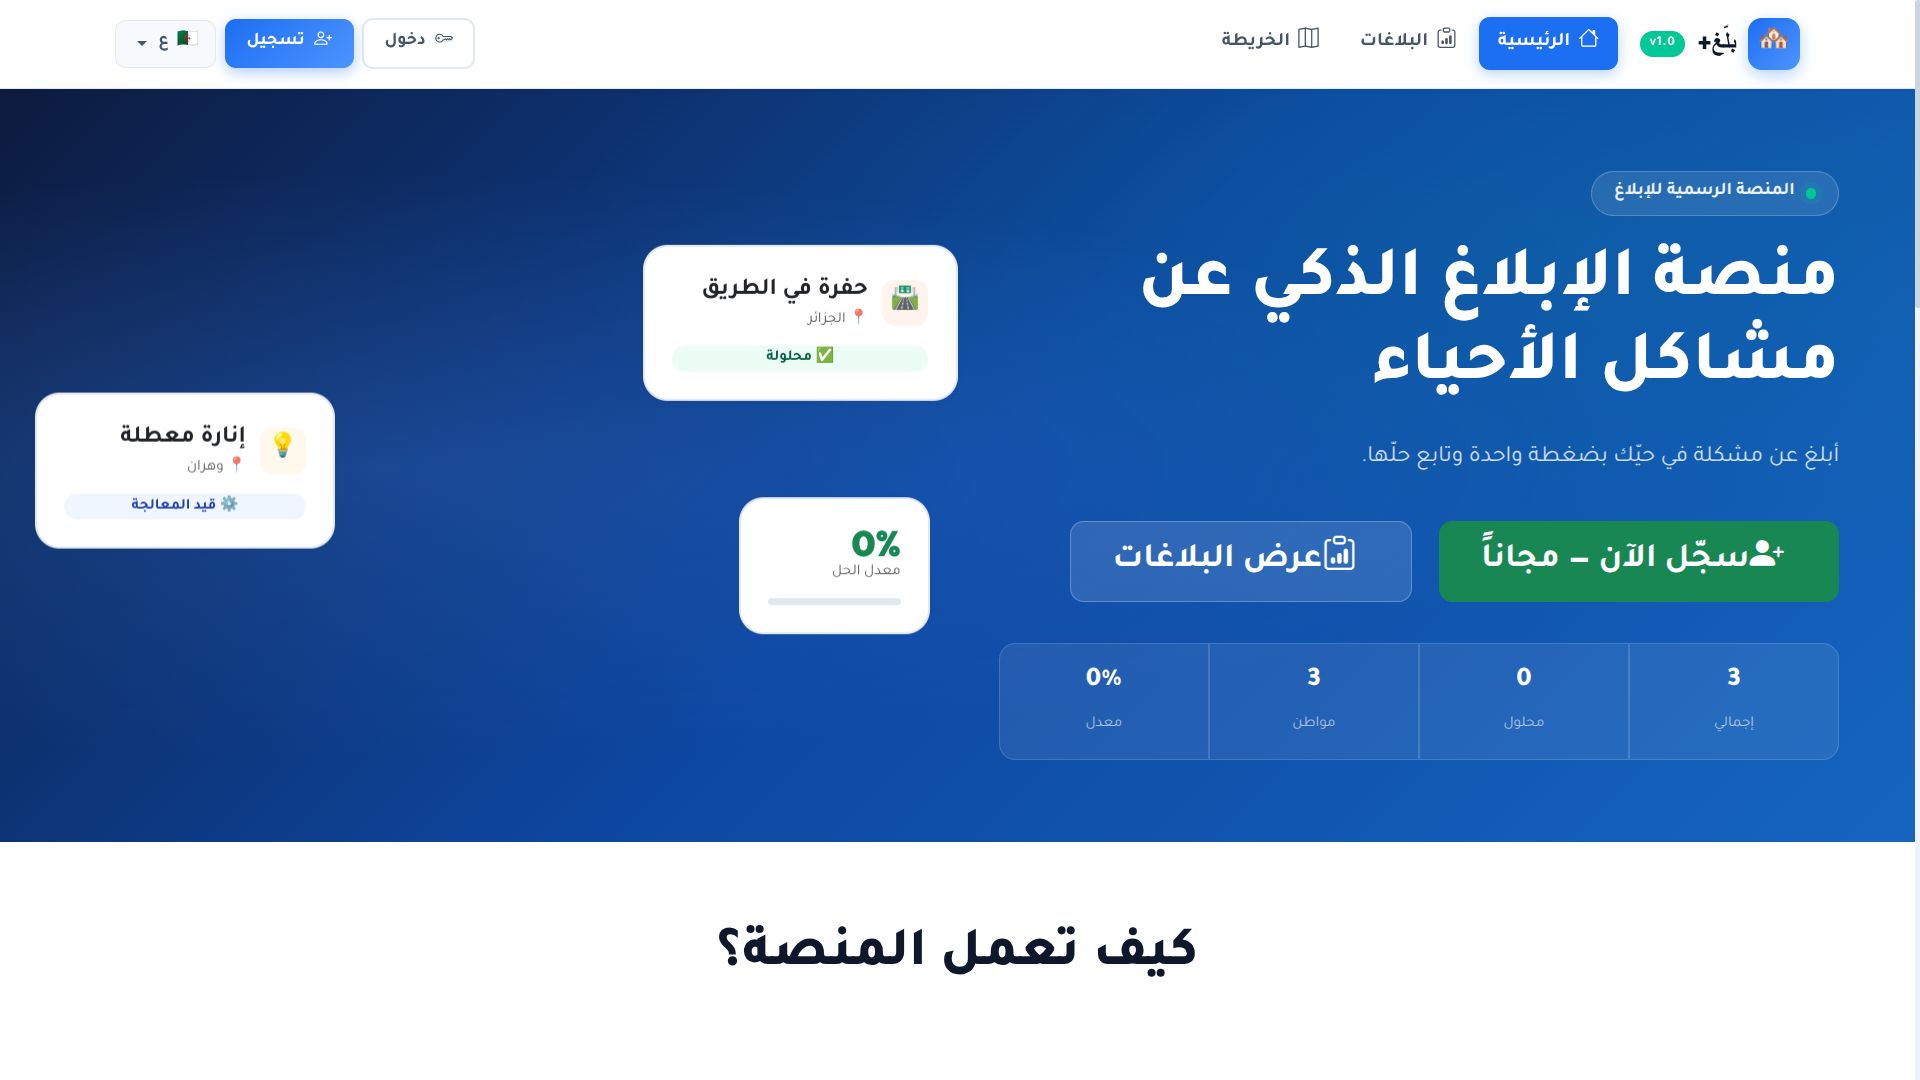
\includegraphics[width=0.85\textwidth]{images/01.png}
  \caption{Interface d'accueil — Page principale de Baligh+}
  \label{fig:accueil}
\end{figure}

\section{Interface de la Carte Interactive}

Cette interface affiche tous les signalements géolocalisés sur une carte
OpenStreetMap interactive (Leaflet.js). Chaque marqueur est coloré selon la
catégorie du signalement. En cliquant sur un marqueur, l'utilisateur voit le
titre, la commune, le statut et un lien vers le détail complet. Un compteur en
haut indique le nombre de signalements localisés. La carte supporte le
clustering automatique pour les zones denses.

\begin{figure}[H]
  \centering
  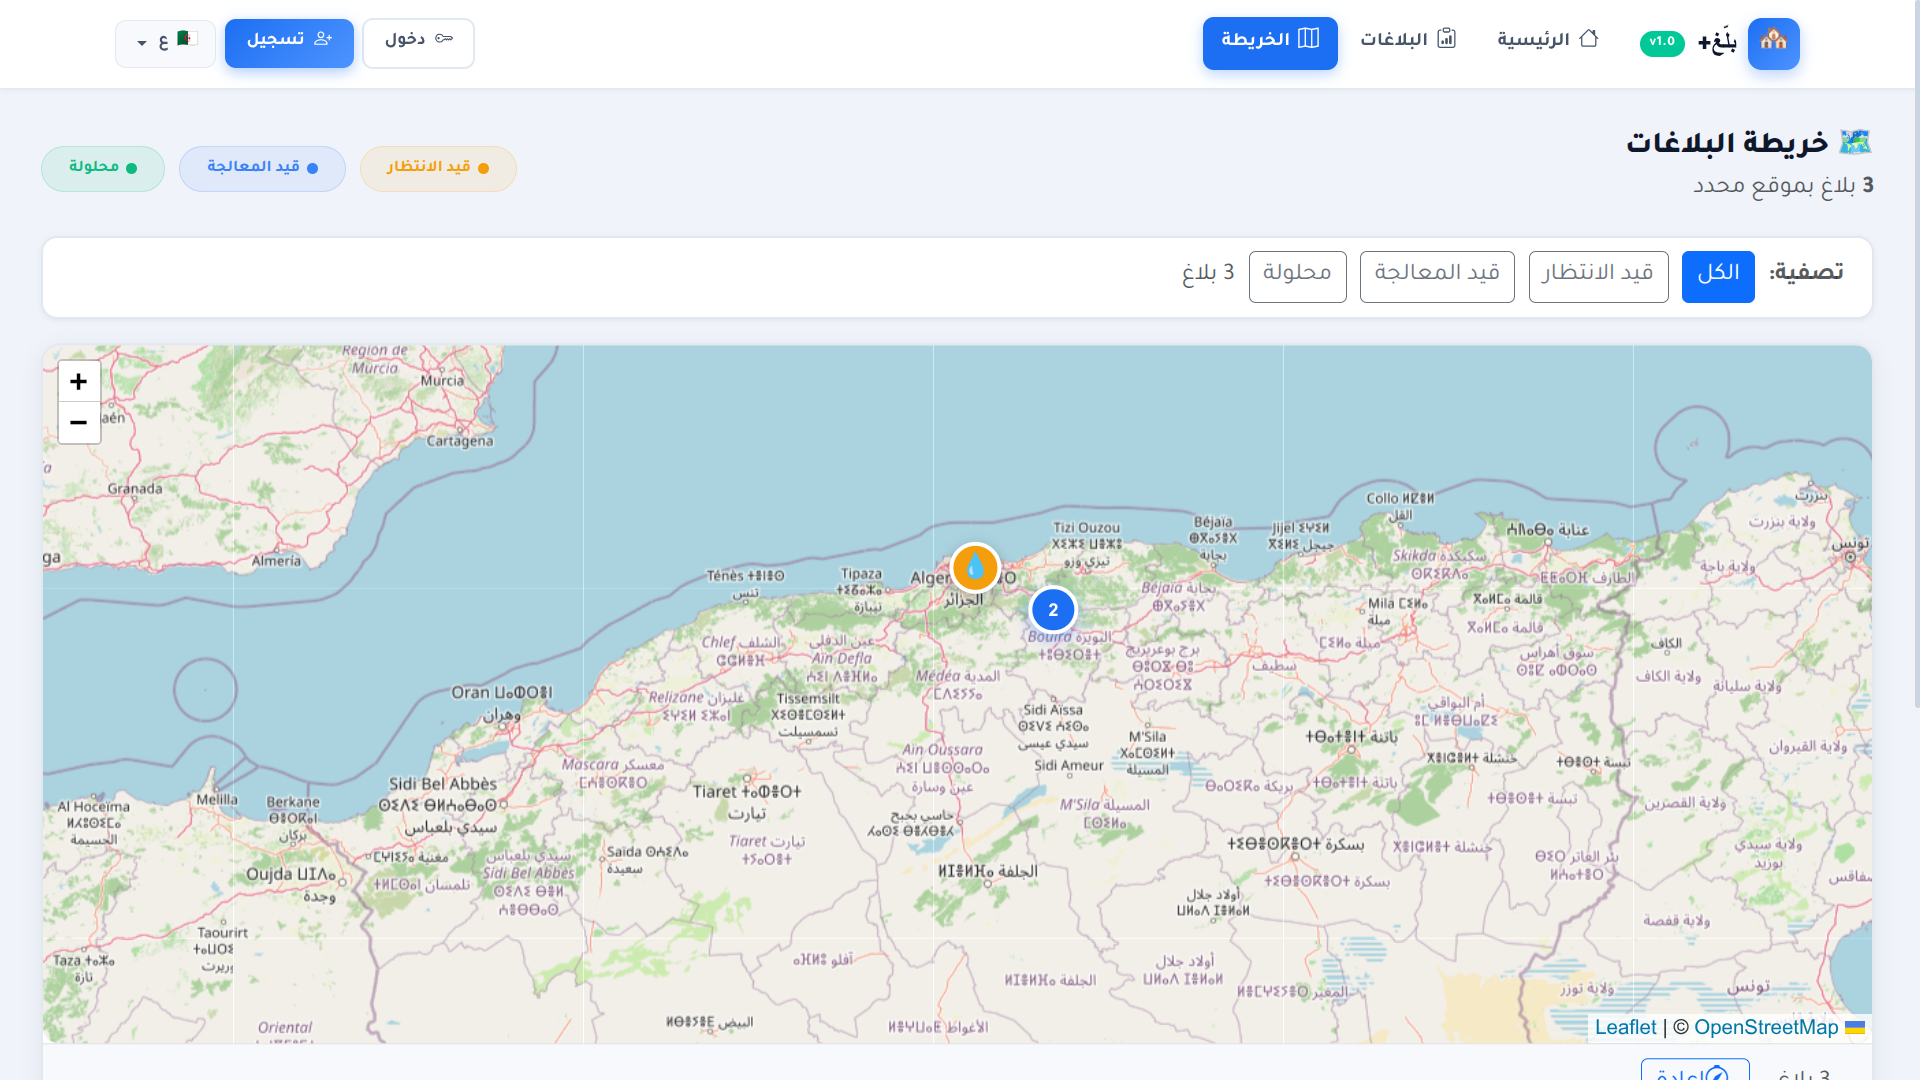
\includegraphics[width=0.90\textwidth]{images/02.png}
  \caption{Carte interactive des signalements géolocalisés}
  \label{fig:carte}
\end{figure}

\section{Interface de Soumission d'un Signalement}

Cette interface guide le citoyen connecté à travers un formulaire structuré
comprenant :
\begin{itemize}
  \item Titre du problème (champ texte, obligatoire).
  \item Type de problème (sélecteur : Route\,/\,Éclairage\,/\,Déchets\,/\,Eau\,/\,Autre).
  \item Wilaya (liste déroulante des 58 wilayas algériennes avec code officiel).
  \item Commune\,/\,Quartier (champ texte avec suggestions).
  \item Description détaillée (lieu, durée, gravité — zone texte).
  \item Géolocalisation : bouton GPS ou clic sur la carte intégrée (déplacement
        du marqueur possible).
  \item Photos (jusqu'à 6 fichiers JPG/PNG/WEBP, interface de glisser-déposer).
  \item Bouton \textit{Envoyer le signalement} — génère le numéro de référence
        et les notifications.
\end{itemize}

\begin{figure}[H]
  \centering
  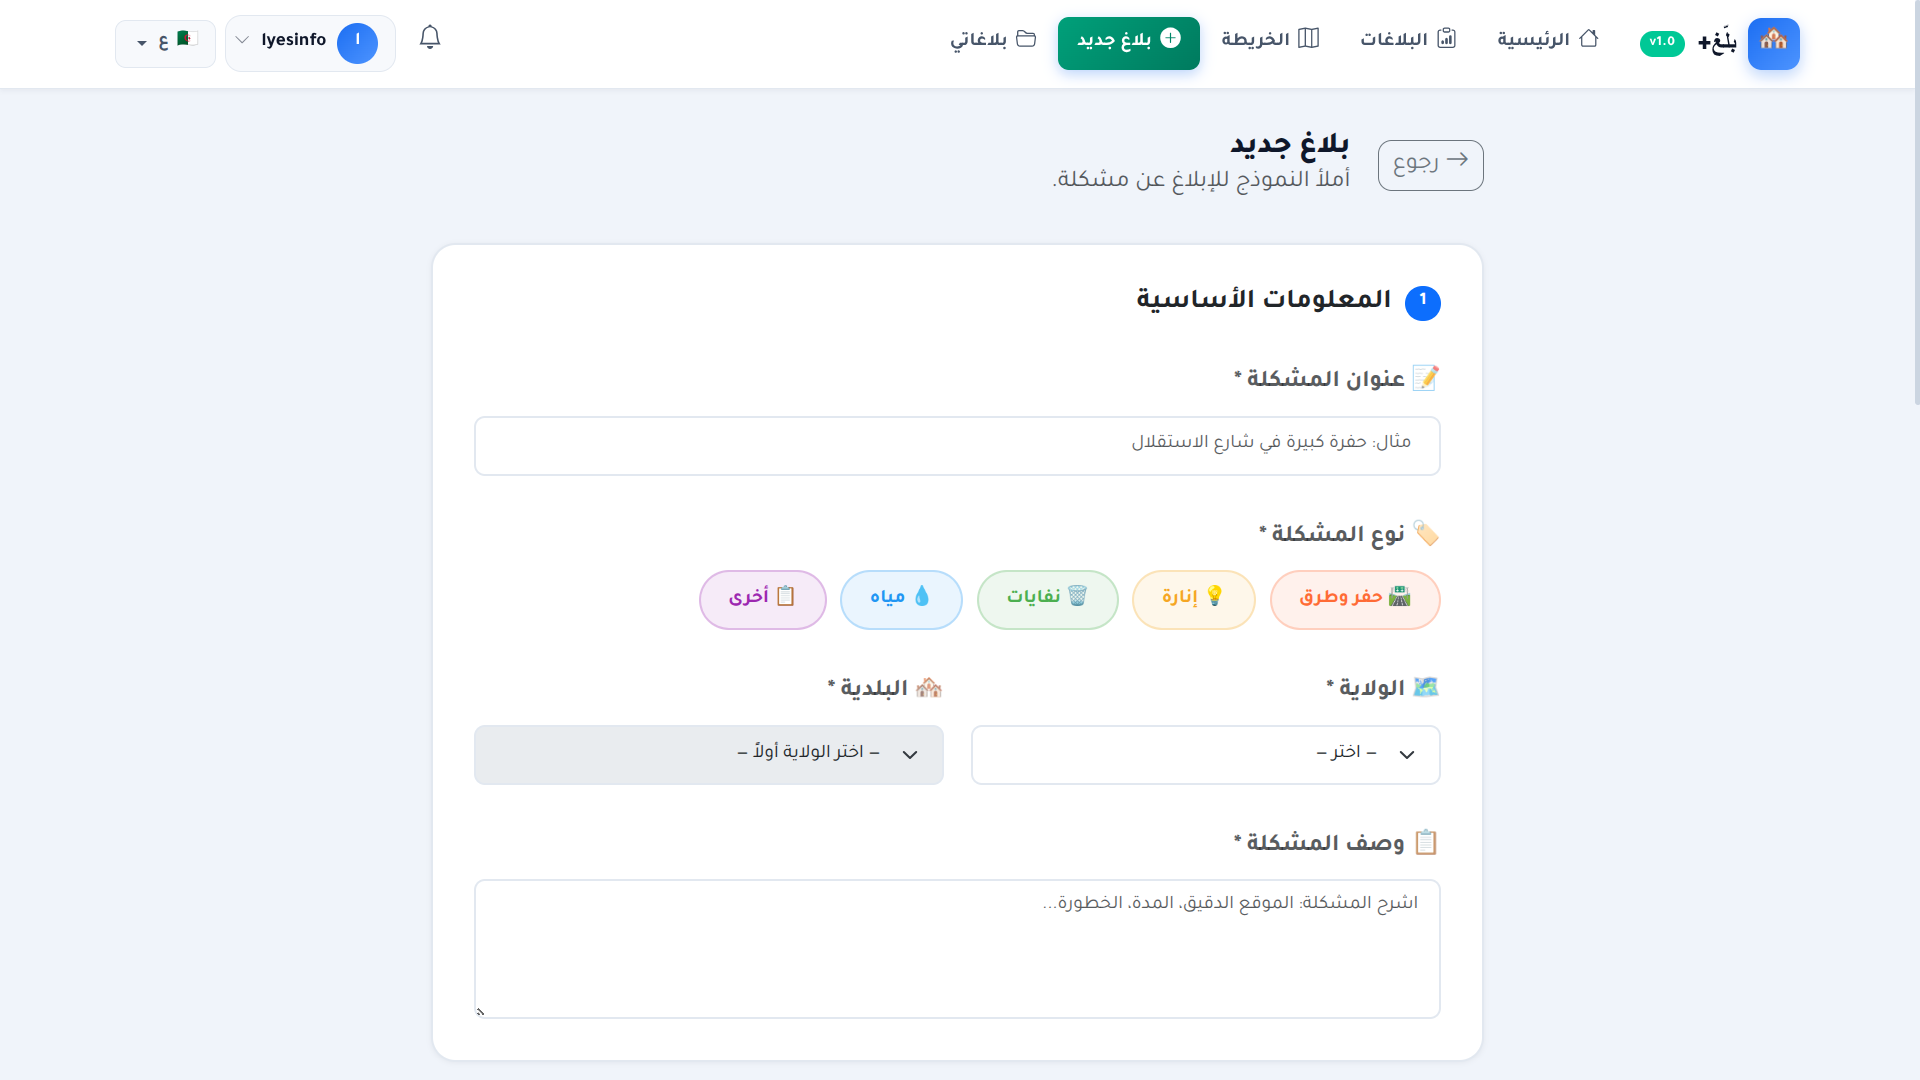
\includegraphics[width=0.85\textwidth]{images/03.png}

  \vspace{0.5cm}

  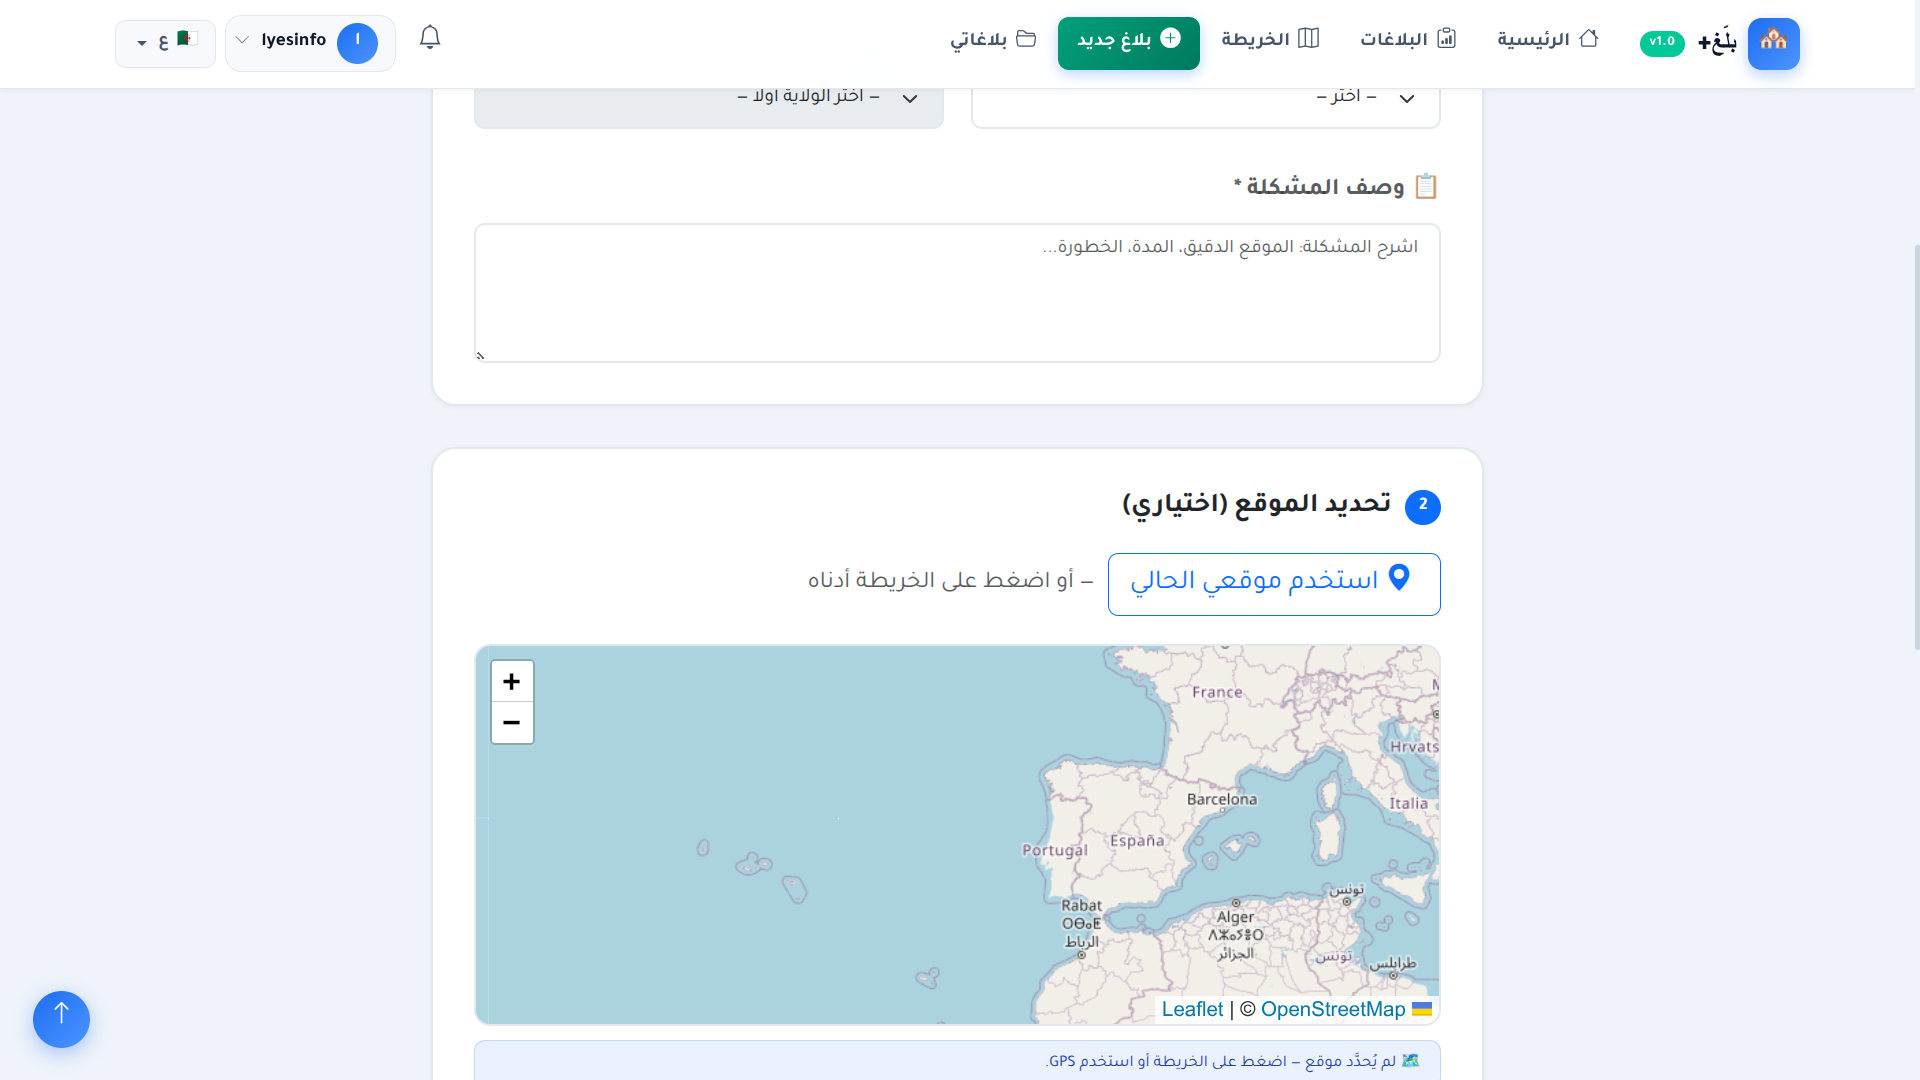
\includegraphics[width=0.85\textwidth]{images/03-01.png}

  \vspace{0.5cm}

  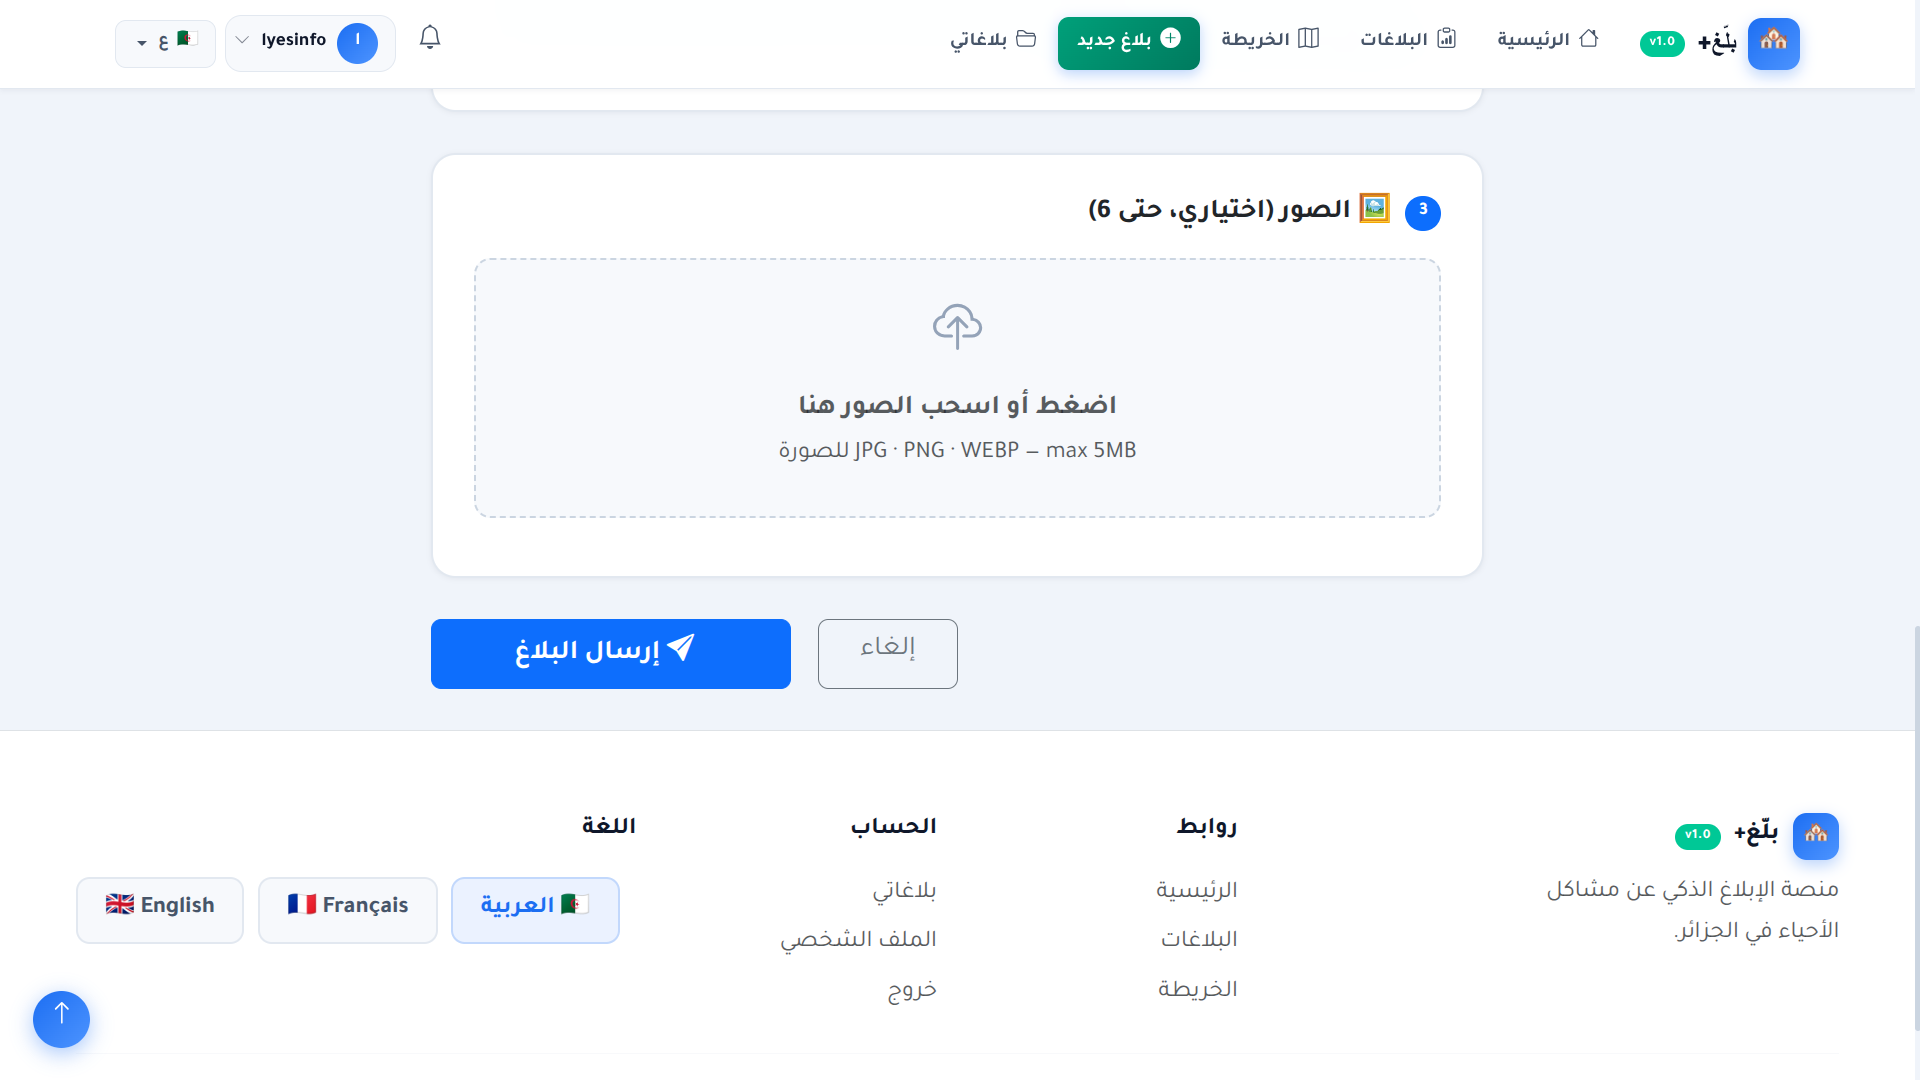
\includegraphics[width=0.85\textwidth]{images/03-03.png}

  \caption{Formulaire de soumission d'un signalement}
  \label{fig:soumission}
\end{figure}

\section{Interface « Tous les signalements »}

Cette page liste l'ensemble des signalements avec filtrage dynamique par statut
(En attente\,/\,En traitement\,/\,Résolu), par catégorie, et recherche plein
texte. Chaque carte de signalement affiche la photo principale, le titre, la
commune, la date, le nombre de votes, le statut coloré et deux boutons : vote
communautaire et accès aux détails.

\begin{figure}[H]
  \centering
  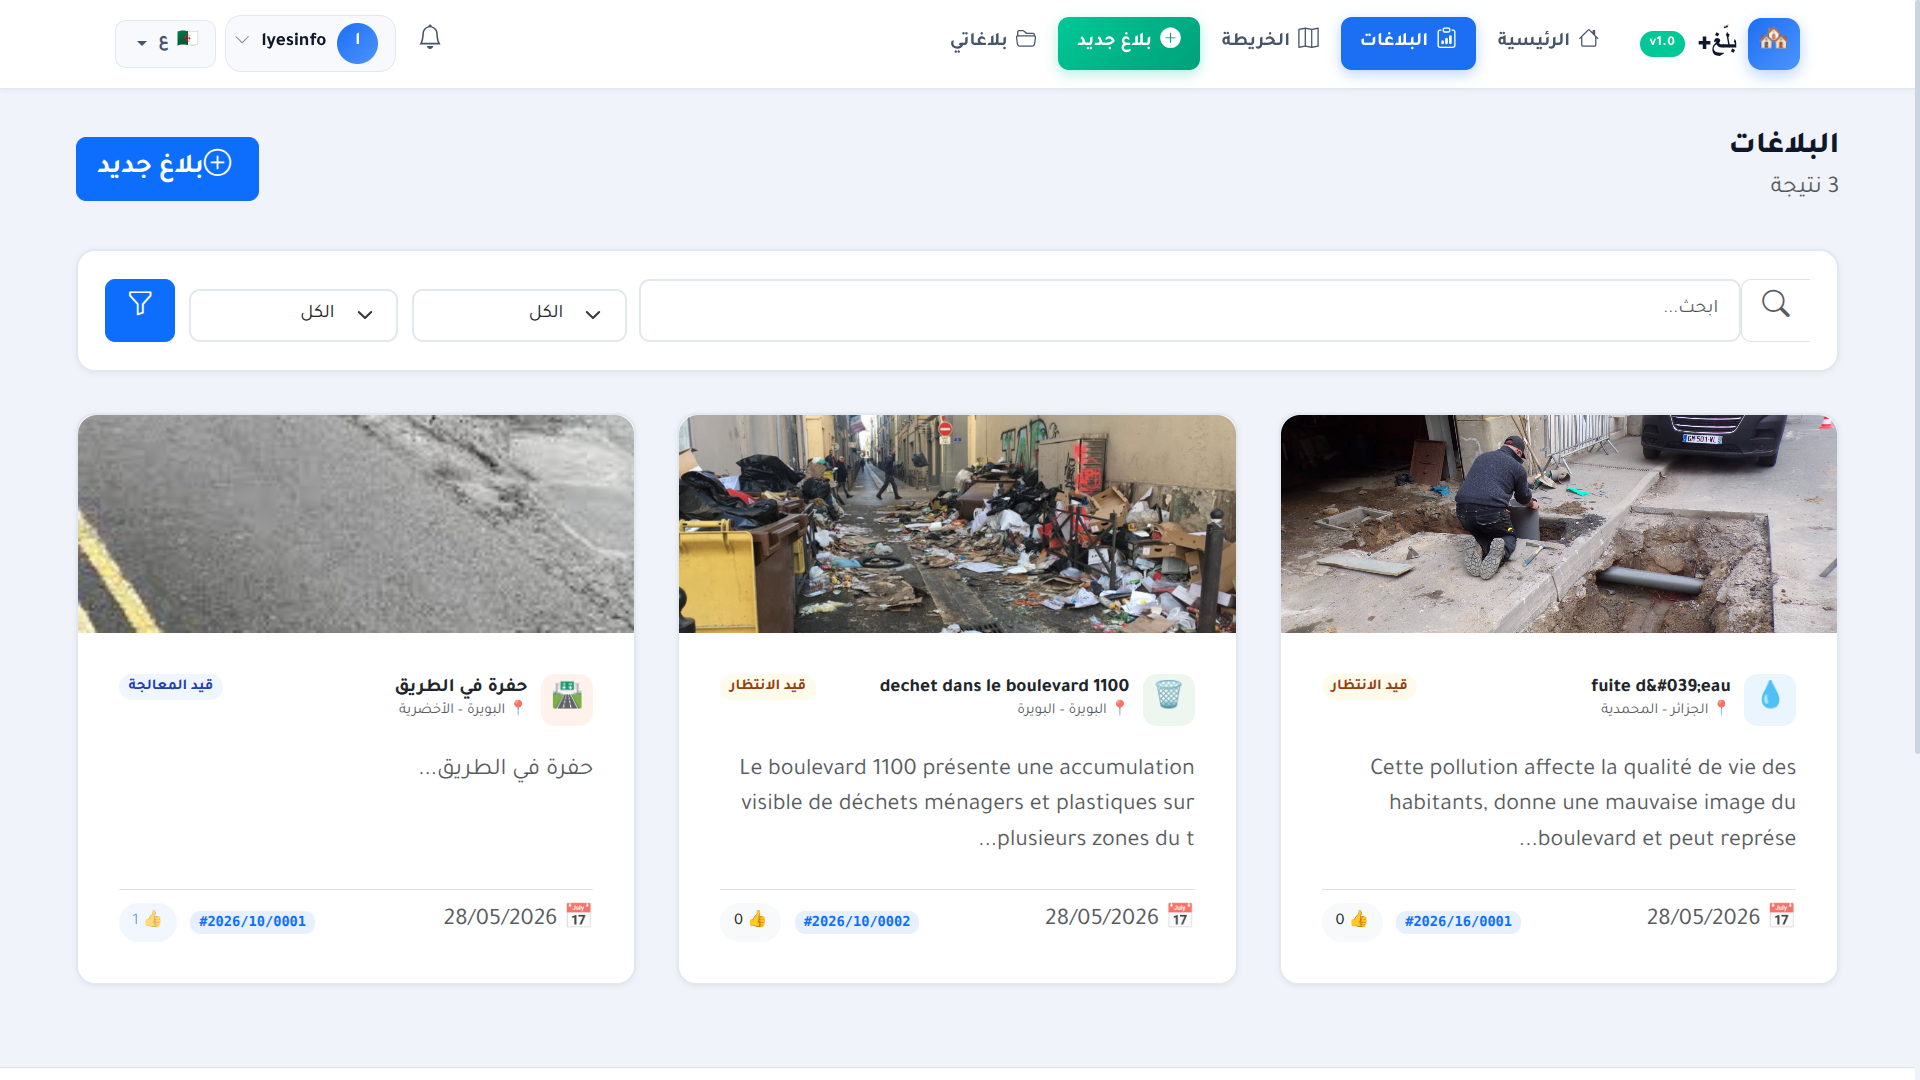
\includegraphics[width=0.90\textwidth]{images/04.png}
  \caption{Liste filtrée de tous les signalements}
  \label{fig:liste}
\end{figure}

\section{Interface de Détail d'un Signalement}

Cette page complète affiche :
\begin{itemize}
  \item Le numéro de référence unique, le titre, la catégorie et la date de
        soumission.
  \item La galerie de photos (jusqu'à 6, avec lightbox navigation clavier).
  \item La description complète et l'historique des changements de statut.
  \item Le bouton de vote communautaire et le compteur de votes.
  \item Le bouton \textit{Voir sur la carte} (modal Leaflet intégré).
  \item La section commentaires avec les réponses officielles distinguées
        visuellement.
  \item Le formulaire d'ajout de commentaire (citoyens connectés uniquement).
\end{itemize}

\begin{figure}[H]
  \centering
  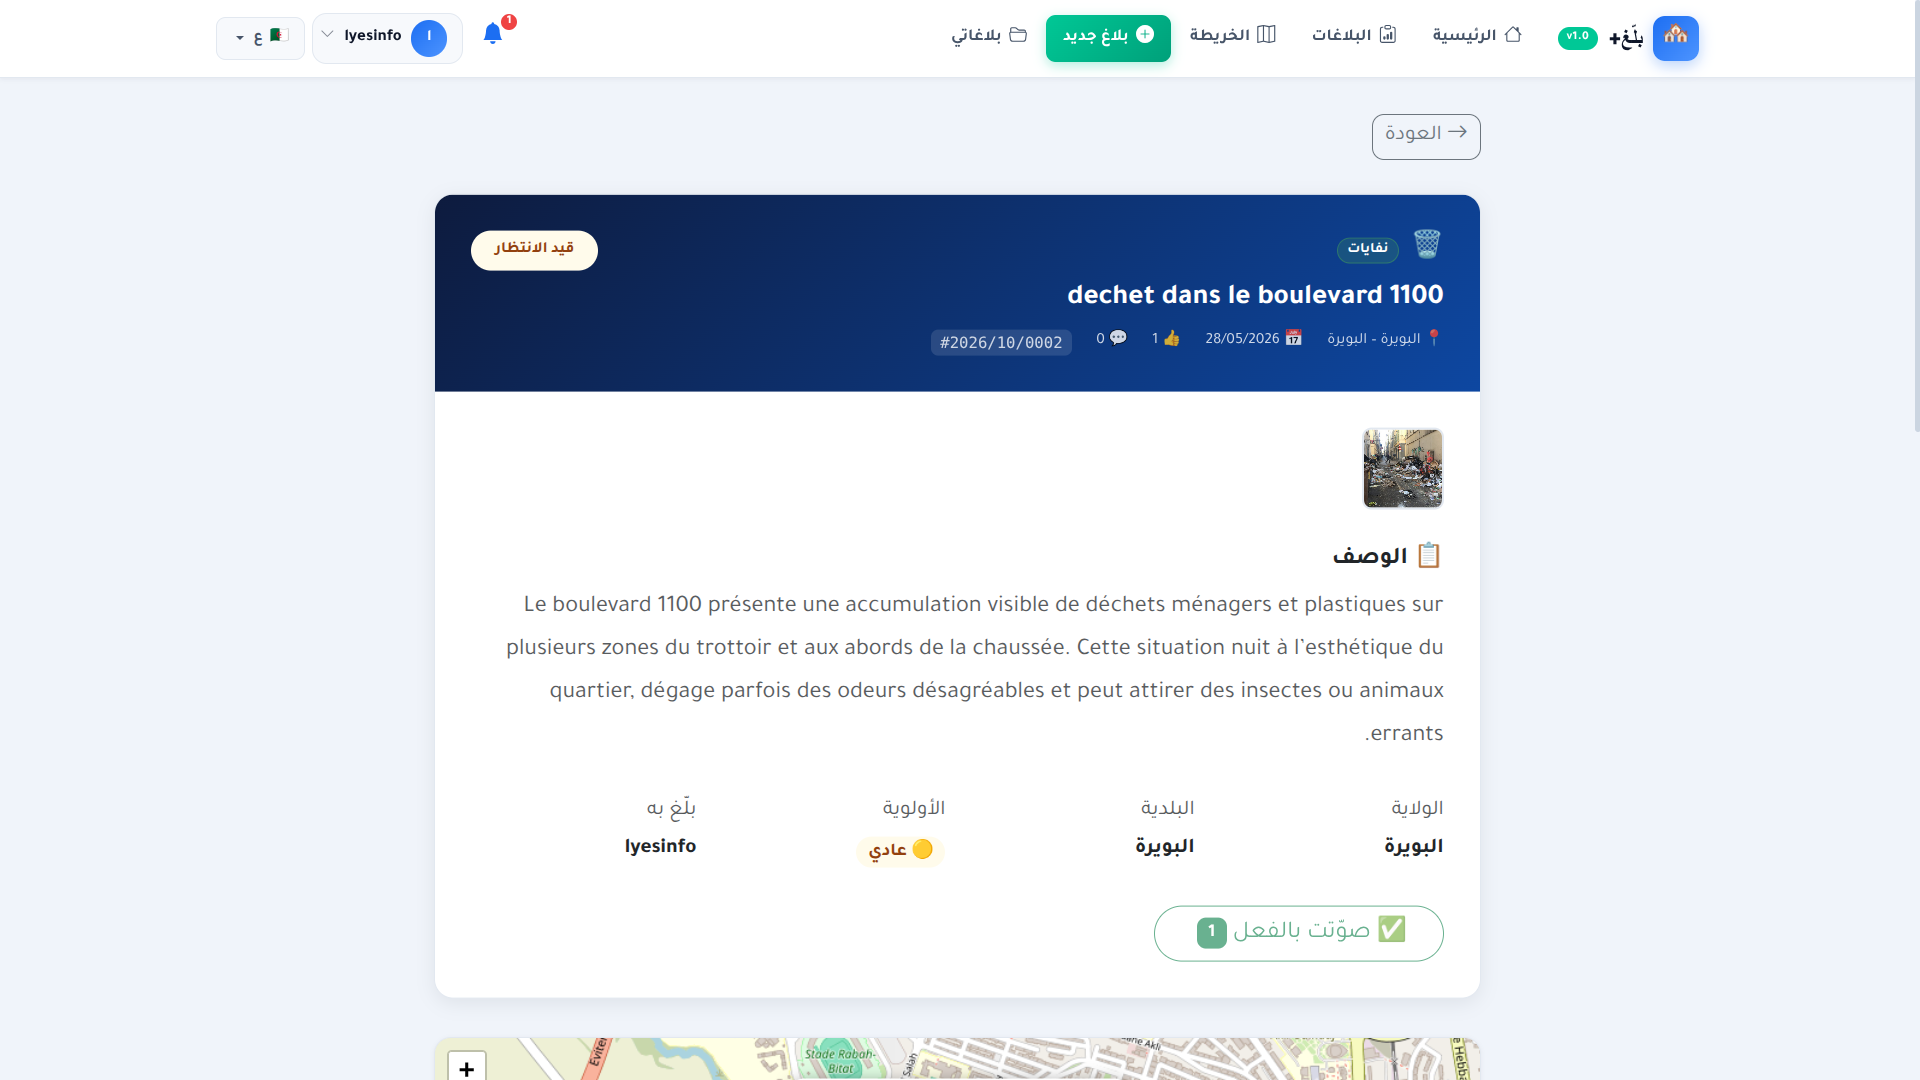
\includegraphics[height=7cm]{images/05.png}
  \hfill
  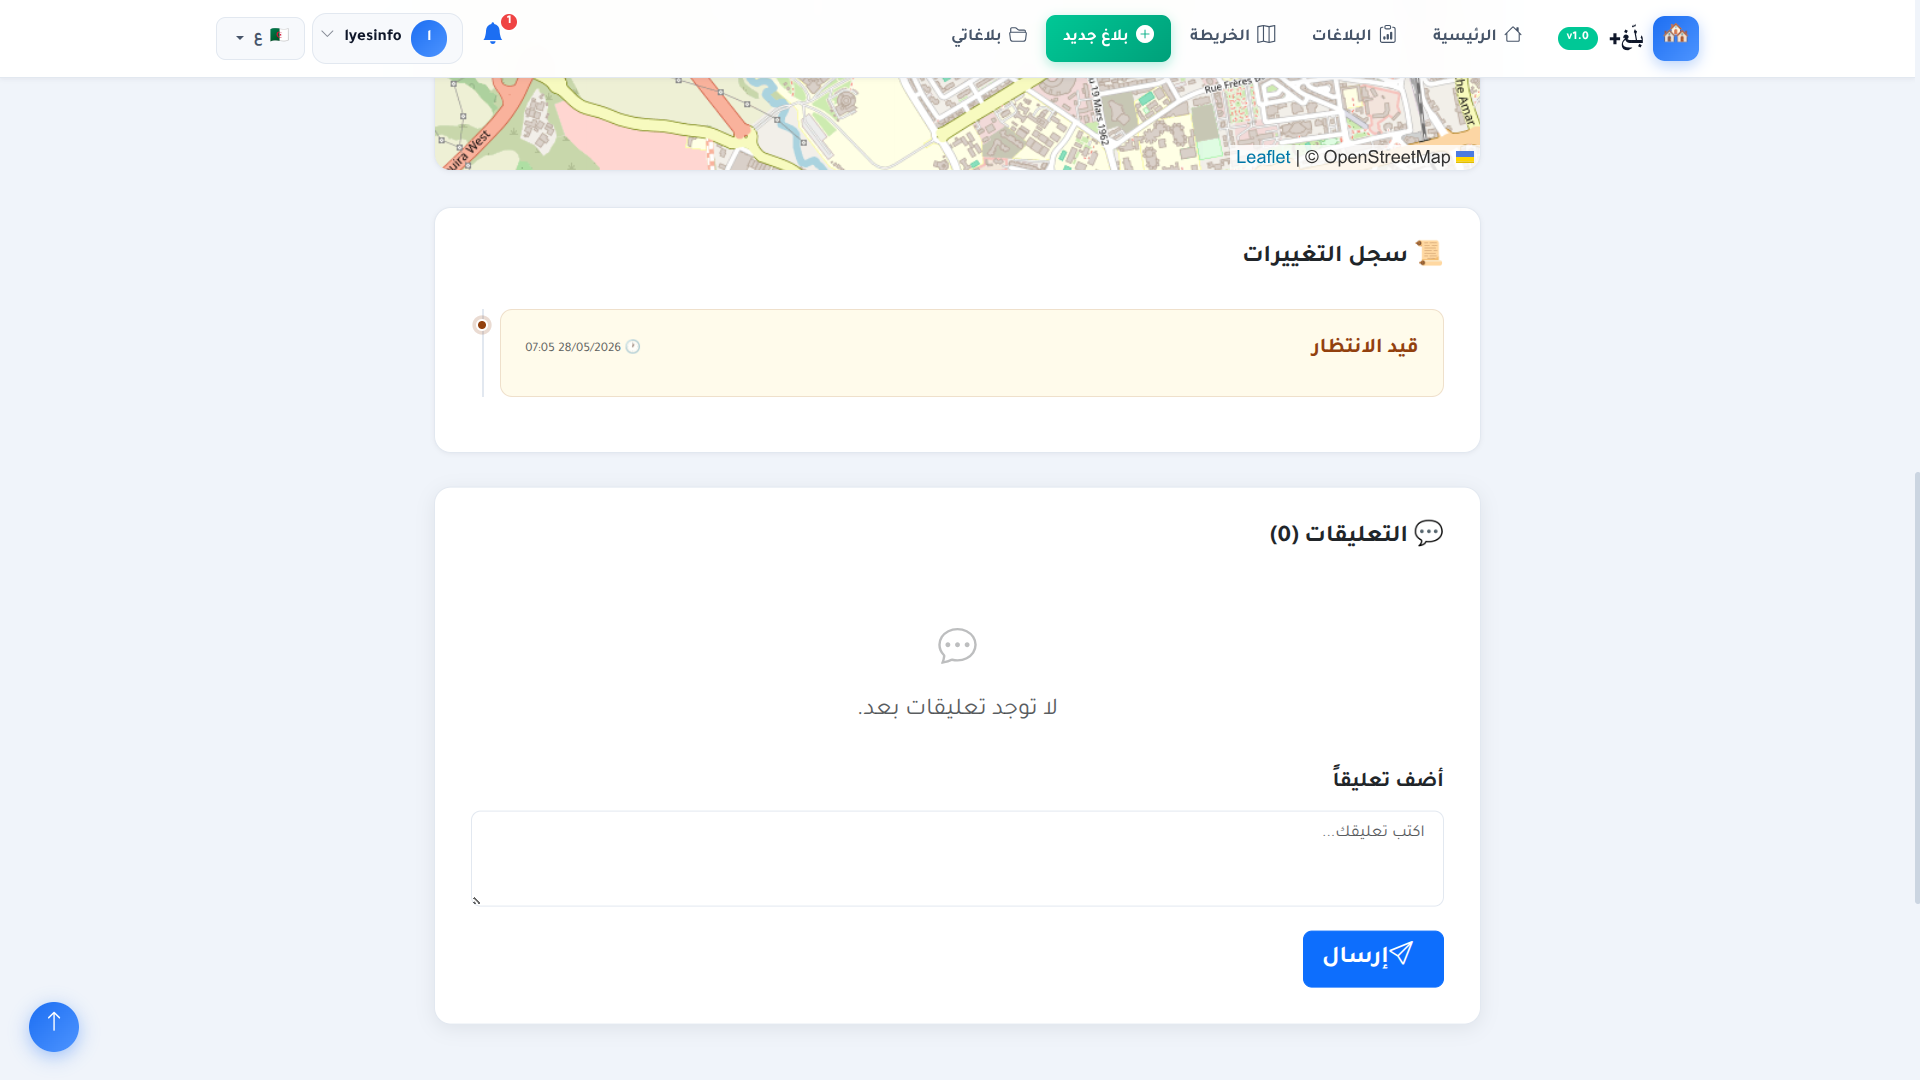
\includegraphics[height=7cm]{images/05-01.png}
  \caption{Page de détail d'un signalement avec commentaires}
  \label{fig:detail}
\end{figure}

\section{Interface de Connexion et d'Inscription}

L'interface de connexion propose deux champs (e-mail\,/\,mot de passe), une
case « Se souvenir de moi » et un lien vers l'inscription. L'interface
d'inscription propose les champs Nom complet, E-mail, Mot de passe (min. 6
caractères) et Confirmation de mot de passe, avec validation côté serveur.

\begin{figure}[H]
  \centering
  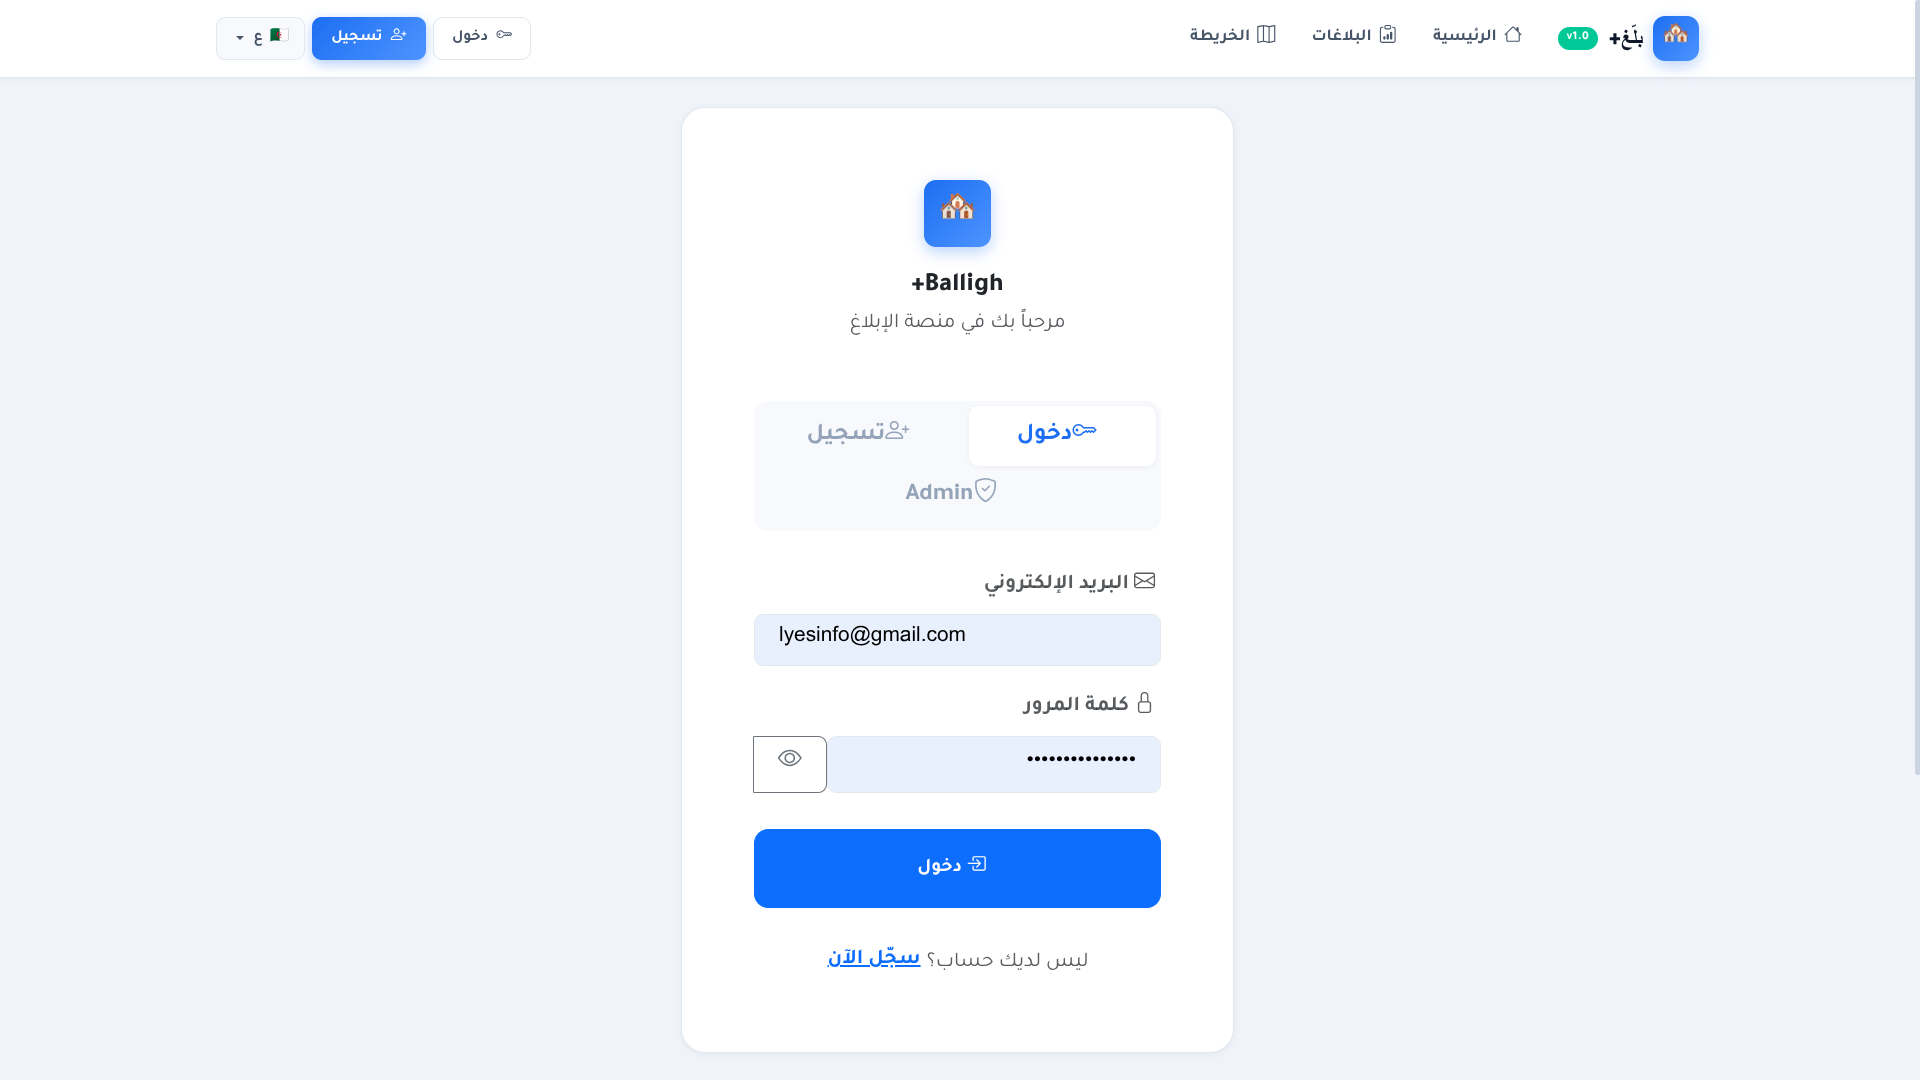
\includegraphics[width=0.90\textwidth]{images/06.png}
  \caption{Interface de connexion et d'inscription}
  \label{fig:connexion}
\end{figure}

\section{Interface « Mes signalements »}

Cette page personnelle liste tous les signalements soumis par l'utilisateur
connecté, avec le statut actuel, le nombre de votes et de commentaires, et des
statistiques récapitulatives (Total\,/\,Résolus). Un bouton \textit{Nouveau
signalement} est mis en évidence pour encourager la contribution.

\begin{figure}[H]
  \centering
  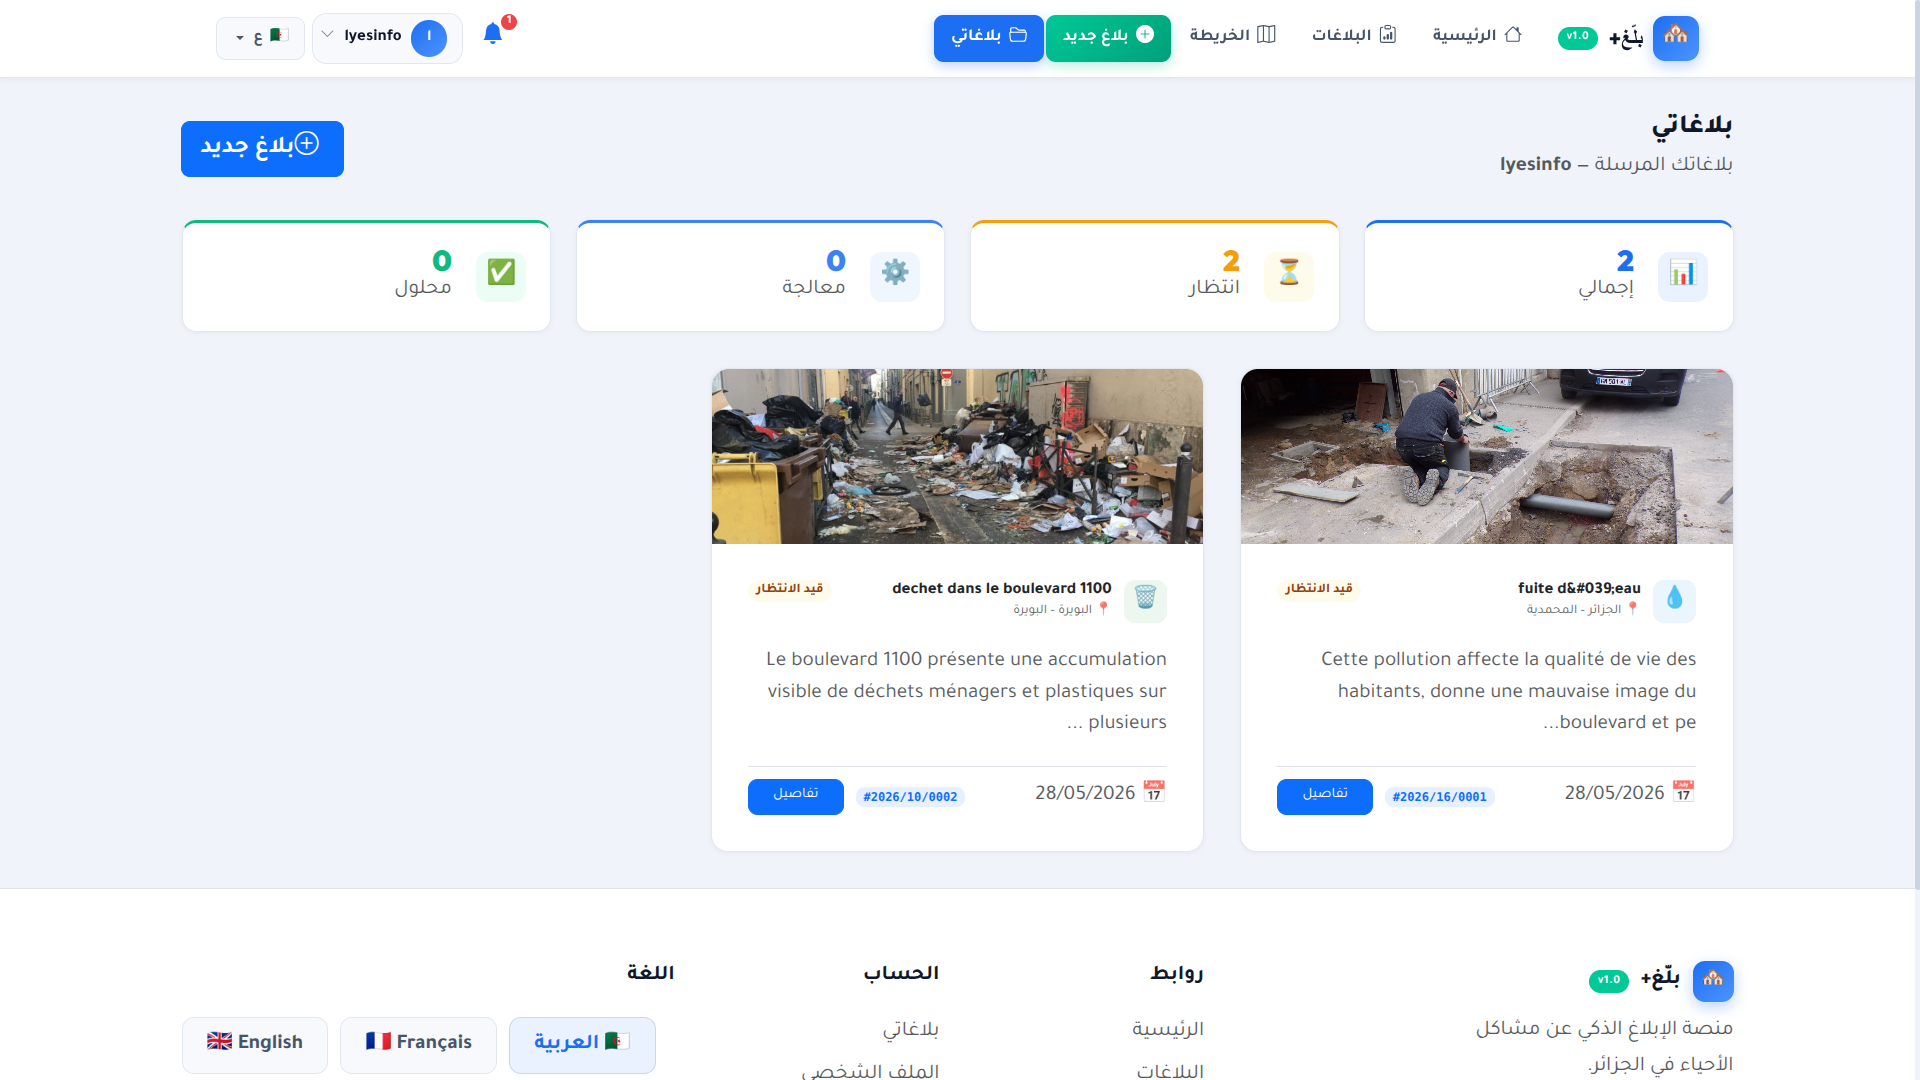
\includegraphics[width=0.90\textwidth]{images/07.png}
  \caption{Interface personnelle « Mes signalements »}
  \label{fig:mes-signalements}
\end{figure}

\section{Interface du Tableau de Bord Administrateur}

L'espace administrateur est accessible via un accès sécurisé (onglet
\textit{Admin} dans l'interface de connexion). Une fois connecté,
l'administrateur dispose d'une barre de navigation dédiée avec les boutons :
\textbf{Accueil}, \textbf{Carte}, \textbf{Export CSV} et \textbf{Déconnexion}.

Le tableau de bord propose une vue complète et structurée de la plateforme :

\subsection{Statistiques globales}
Des compteurs en temps réel affichent le nombre total de signalements, ceux
\textit{en attente}, \textit{en traitement}, \textit{résolus} ainsi que le
taux de résolution global (en pourcentage).

\begin{figure}[H]
  \centering
  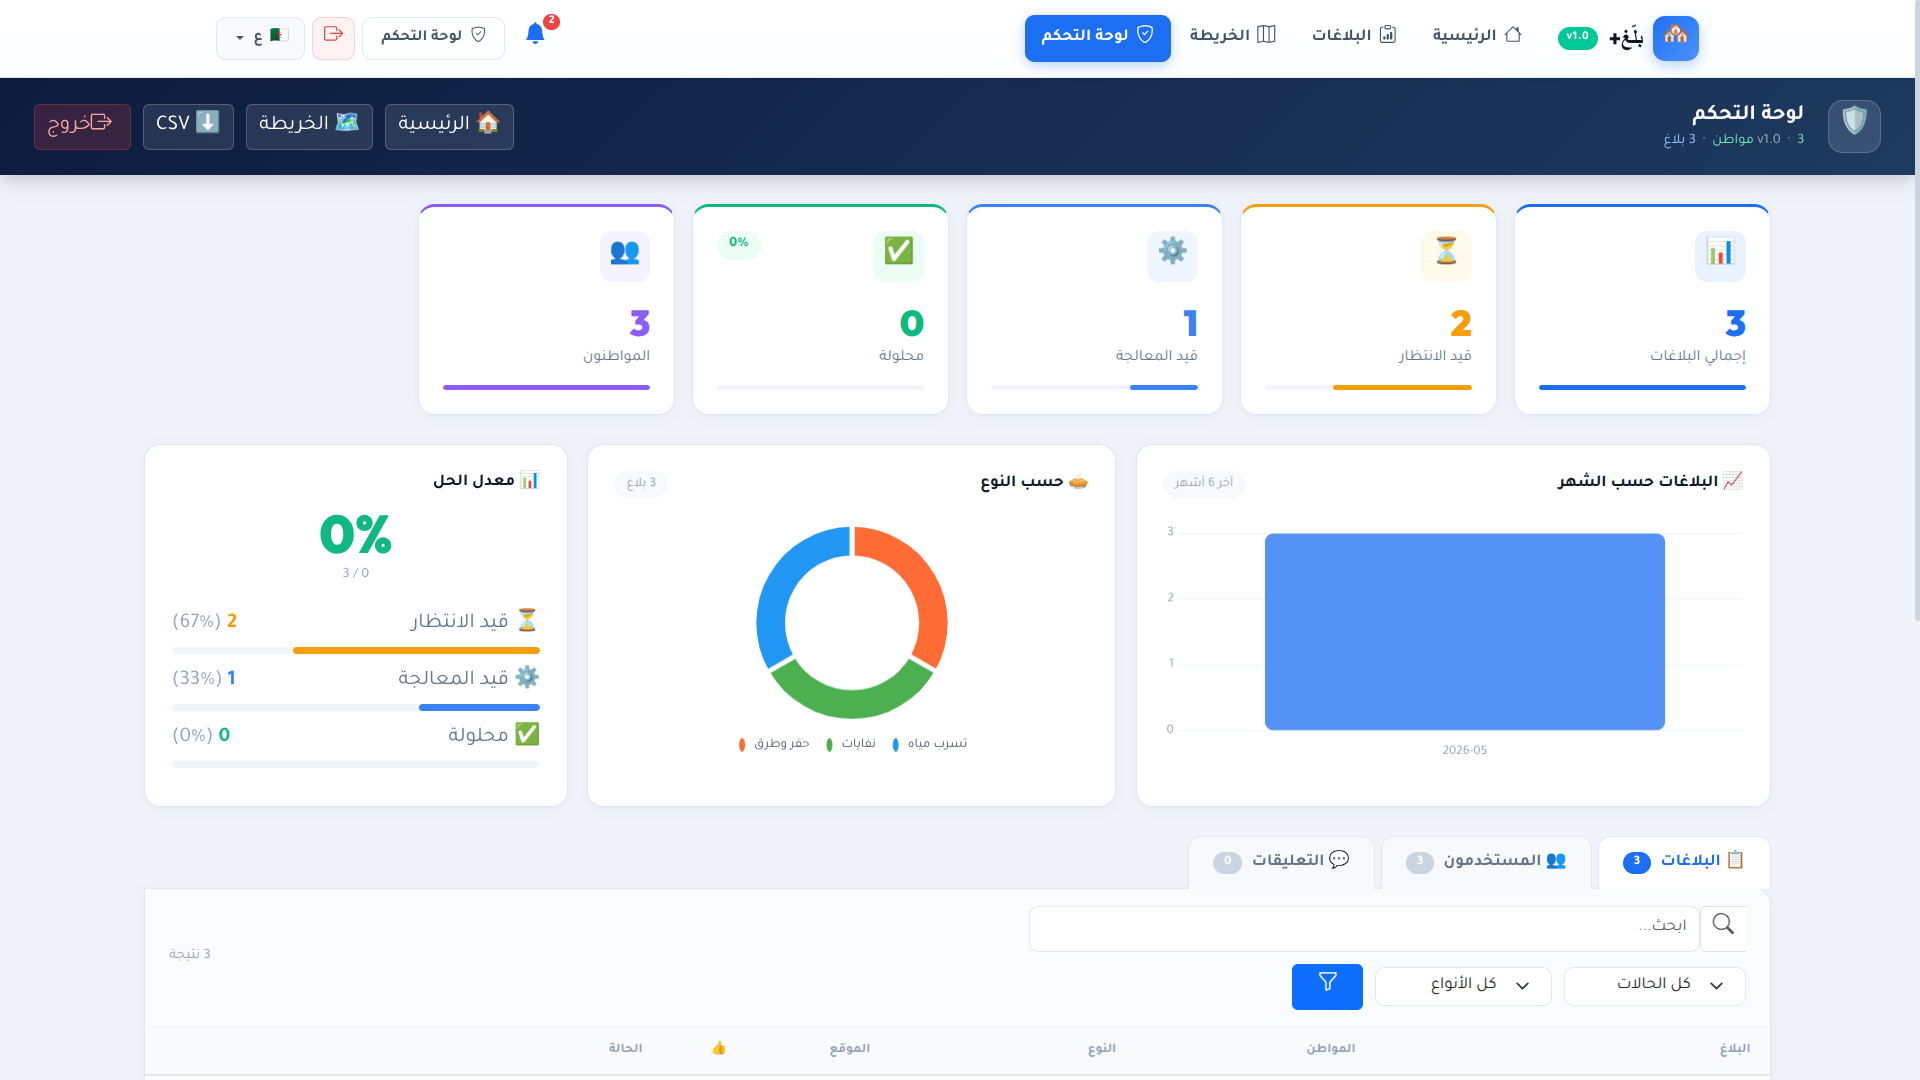
\includegraphics[width=0.90\textwidth]{images/admin01.png}
  \caption{Statistiques globales}
  \label{fig:statistiques-globales}
\end{figure}

\subsection{Visualisation graphique}
Deux graphiques synthétisent l'activité de la plateforme :
\begin{itemize}
  \item \textbf{Répartition par catégorie} : graphique coloré distinguant les
        types de signalements (Trous et routes, Déchets, Fuite d'eau, etc.).
  \item \textbf{Évolution mensuelle} : courbe montrant la progression des
        signalements dans le temps (par exemple mai 2026).
\end{itemize}

\subsection{Gestion des signalements}
L'onglet \textbf{Signalements} (3 résultats dans l'exemple) présente une liste
paginée avec pour chaque entrée :
\begin{itemize}
  \item Le titre du signalement et son numéro de référence unique (ex.
        \texttt{\#2026/16/0001}).
  \item Le nom du citoyen déclarant et son avatar.
  \item Le type de problème avec badge coloré (Fuite d'eau, Déchets, Trous et
        routes\ldots).
  \item La localisation (wilaya\,/\,commune).
  \item Le nombre de votes communautaires.
  \item La date de soumission.
  \item Deux menus déroulants inline pour modifier le \textbf{statut} (En
        attente, En traitement, Résolu) et la \textbf{priorité} (Normale,
        Urgente).
  \item Des boutons d'action rapide : \textit{voir le détail} et
        \textit{supprimer}.
\end{itemize}

\subsection{Gestion des utilisateurs et commentaires}
Deux onglets supplémentaires permettent :
\begin{itemize}
  \item \textbf{Utilisateurs} (3) : liste des comptes enregistrés avec options
        de suspension\,/\,réactivation et suppression.
  \item \textbf{Commentaires} (0) : modération des commentaires soumis par les
        citoyens.
\end{itemize}

\subsection{Export et navigation}
Un bouton \textbf{Export CSV} génère un fichier horodaté de tous les
signalements (compatible Excel UTF-8). Un accès direct à la \textbf{carte
interactive} est disponible depuis la barre de navigation admin. Une icône de
notification en haut à gauche affiche les alertes en temps réel (badge
numérique).

\begin{figure}[H]
  \centering
  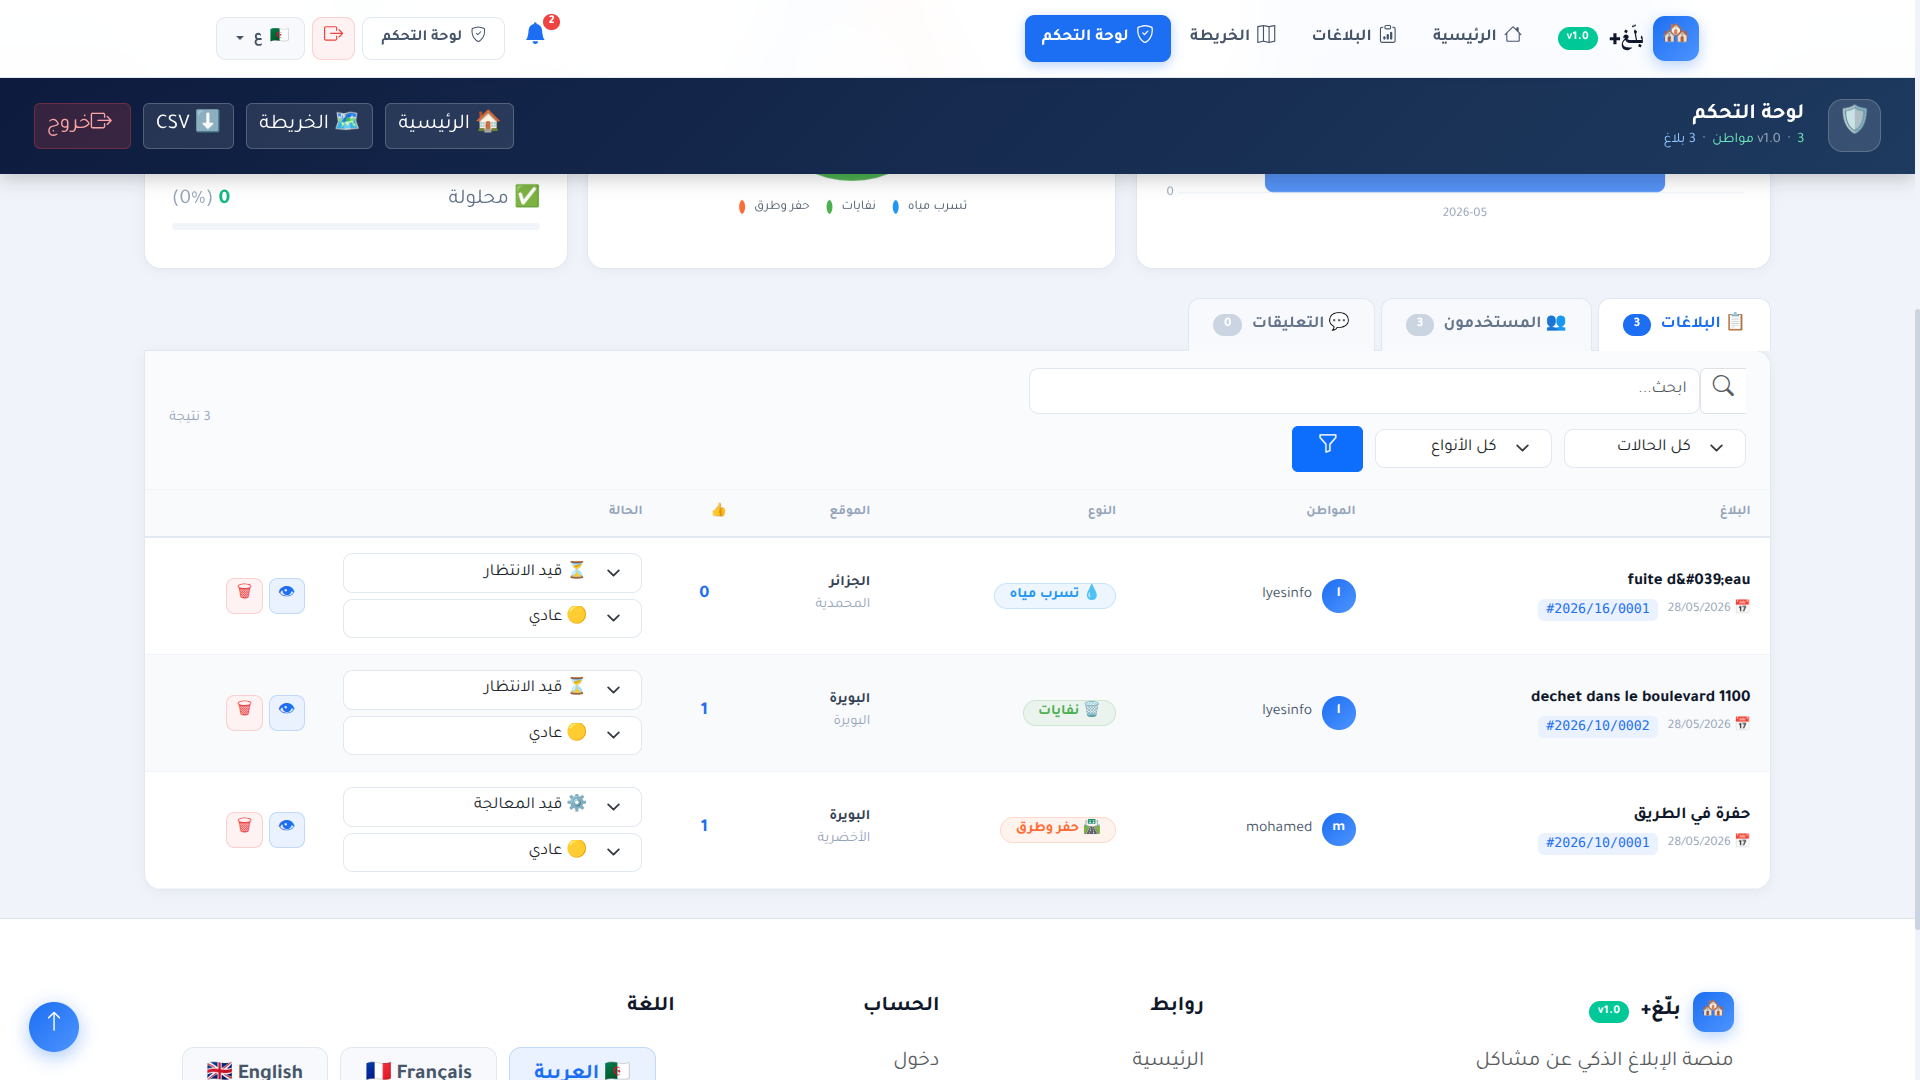
\includegraphics[width=0.90\textwidth]{images/admin02.png}
  \caption{Tableau de bord administrateur — gestion des signalements}
  \label{fig:admin}
\end{figure}

\section{Interface de Profil Utilisateur}

La page profil affiche les informations de l'utilisateur (nom, e-mail, date
d'inscription) et ses statistiques (nombre de signalements, nombre de résolus,
nombre de commentaires). Une section permet de changer le mot de passe avec
validation des trois champs (ancien, nouveau, confirmation).

\begin{figure}[H]
  \centering
  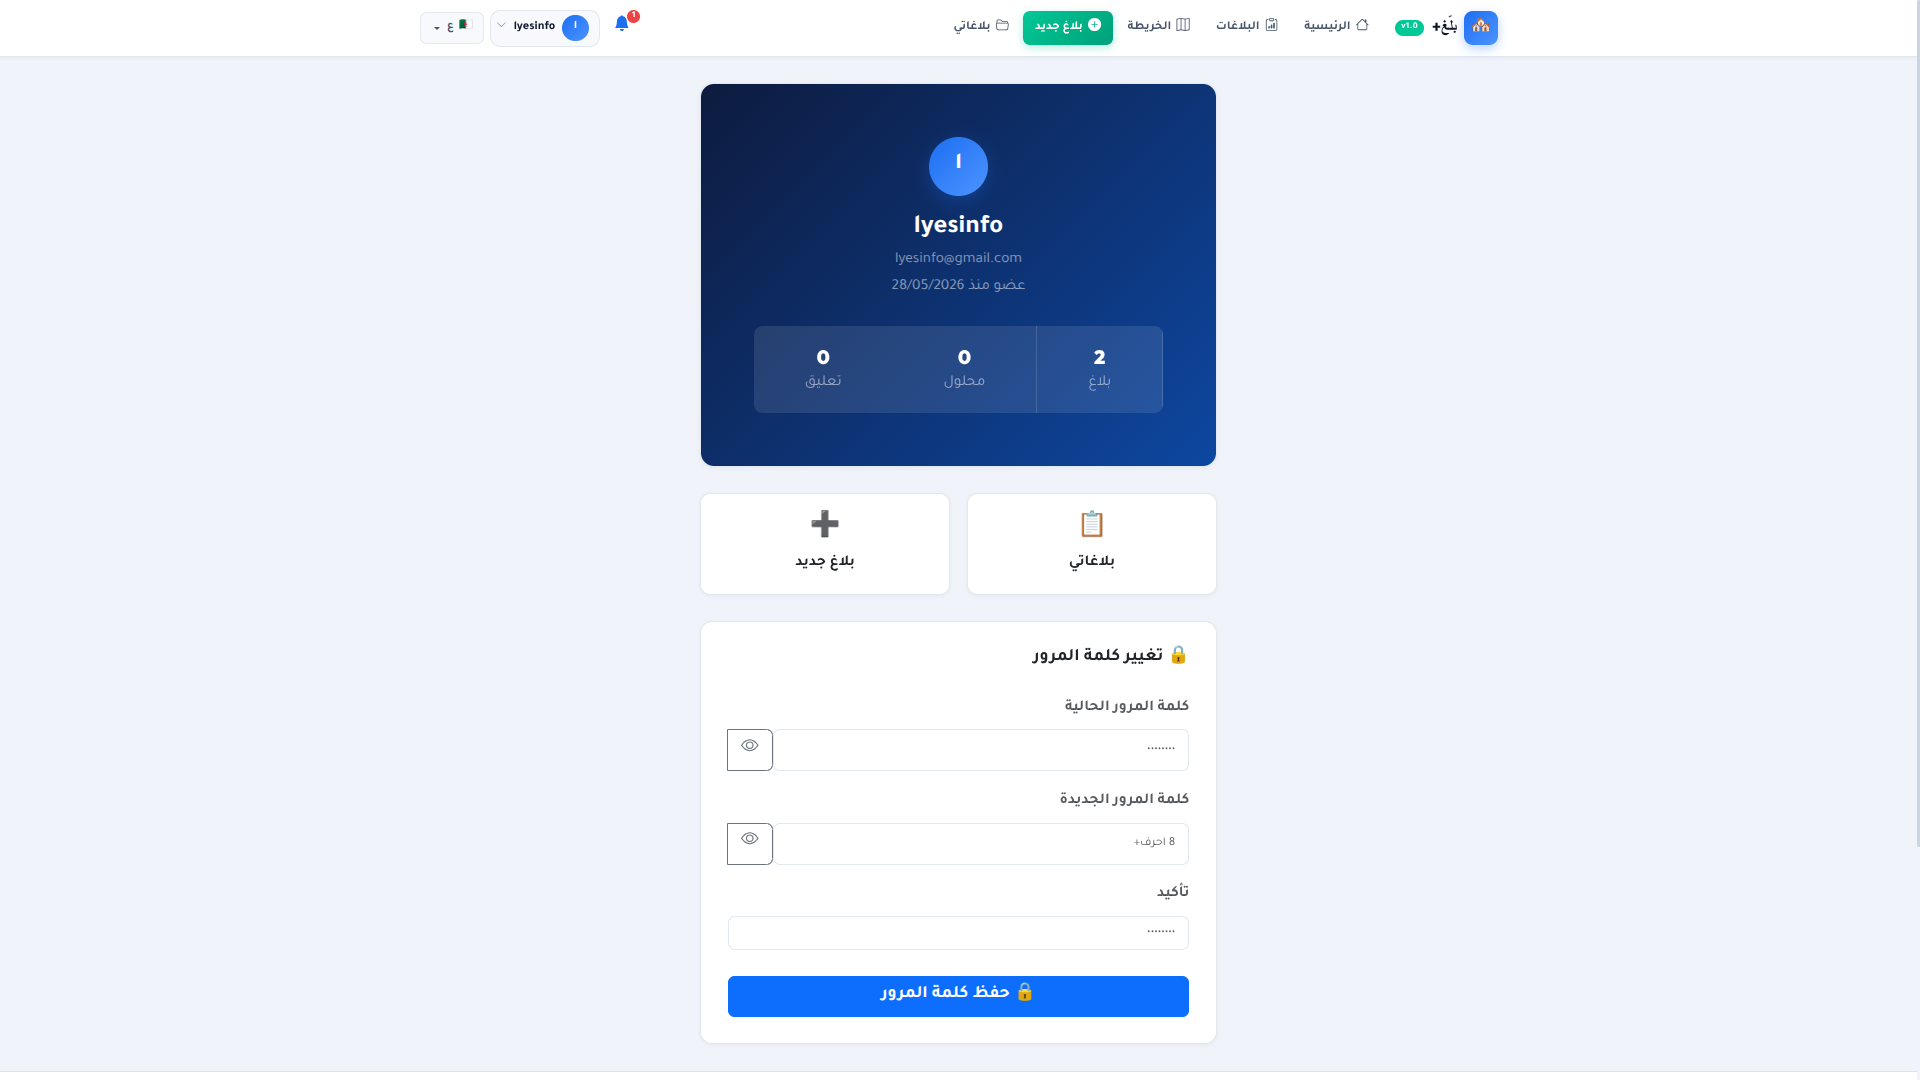
\includegraphics[width=0.90\textwidth]{images/profil01.png}
  \caption{Interface de profil utilisateur}
  \label{fig:profil}
\end{figure}

\section{Système de Notifications}

Le système de notifications en temps quasi-réel fonctionne ainsi :
\begin{itemize}
  \item Une icône cloche dans la navbar affiche le nombre de notifications non
        lues.
  \item Un panneau déroulant liste les notifications (nouveau signalement, vote,
        mise à jour de statut, commentaire officiel) avec icônes distinctives.
  \item Les notifications non lues sont mises en évidence par un point coloré.
  \item Le bouton « Tout marquer comme lu » efface les indicateurs.
  \item Actualisation automatique toutes les 30 secondes
        (\texttt{setInterval}).
\end{itemize}

\begin{figure}[H]
  \centering
  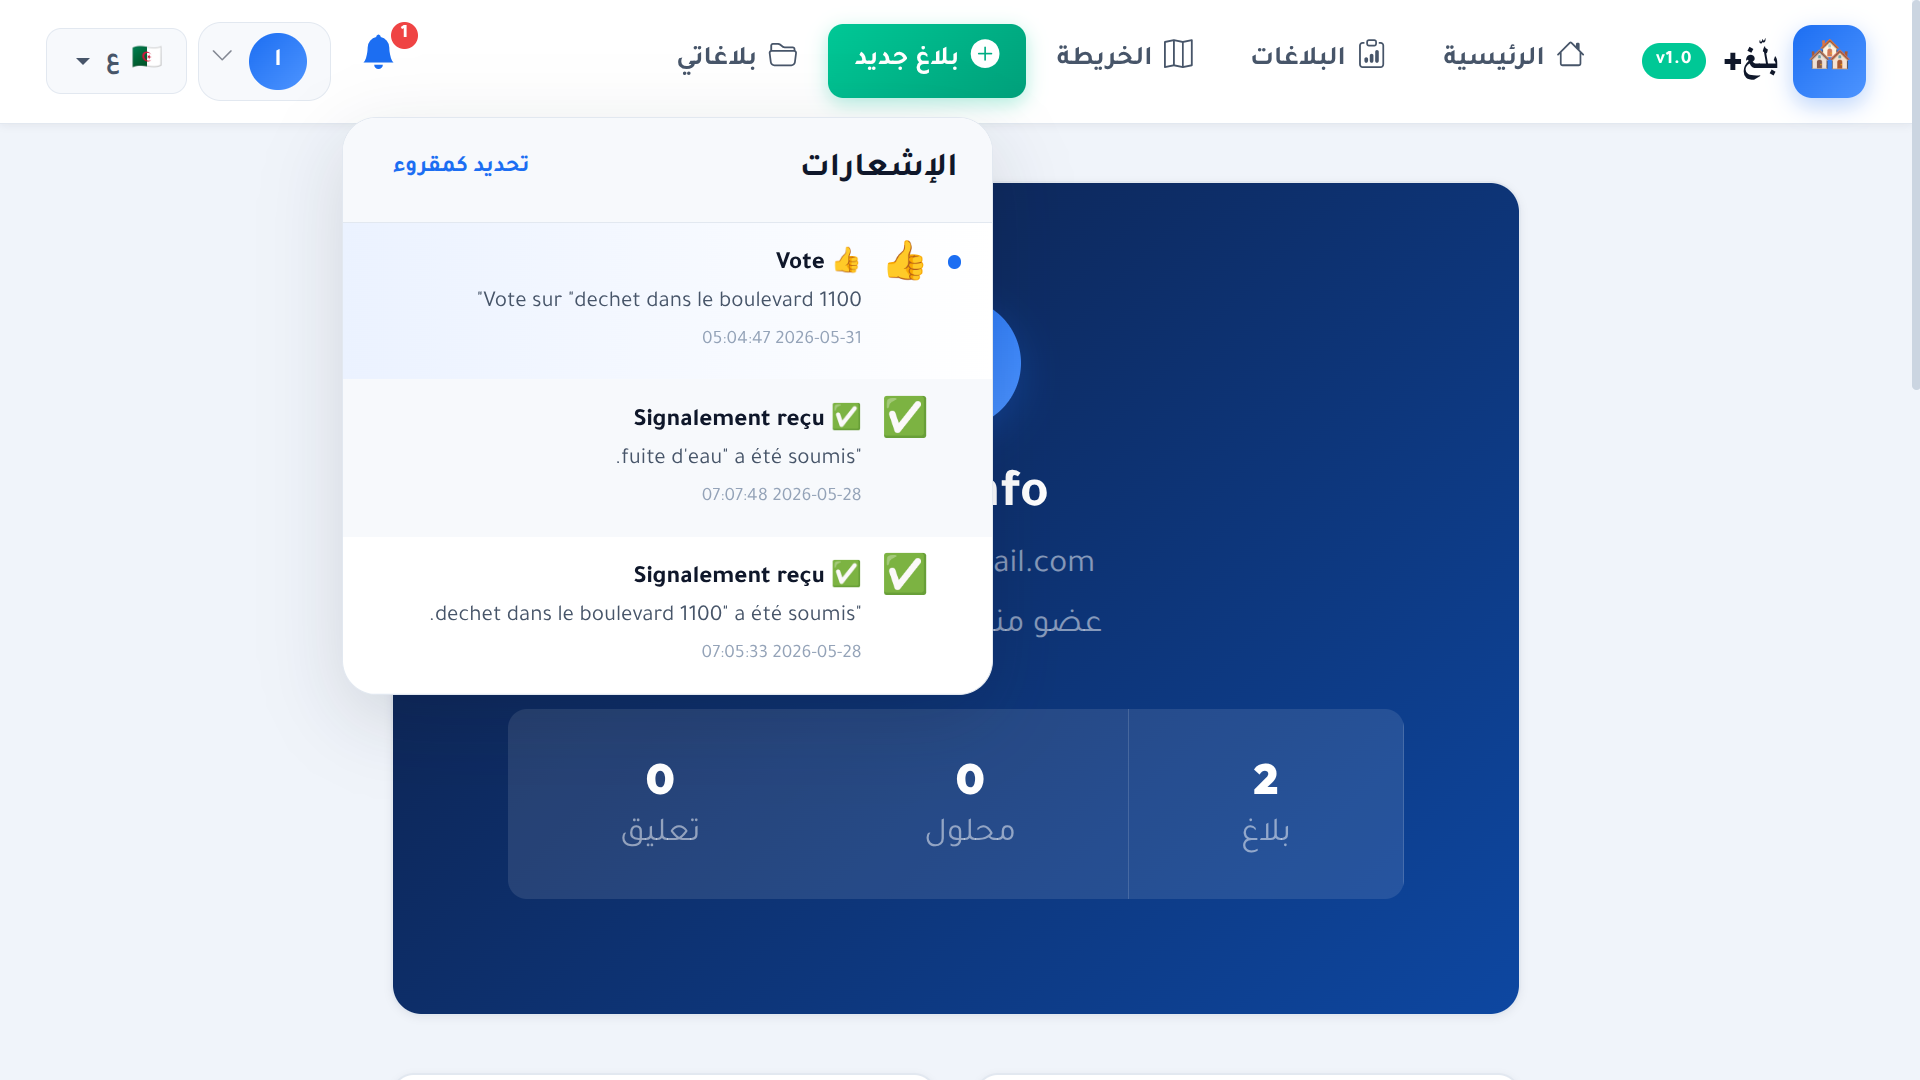
\includegraphics[width=0.90\textwidth]{images/notification.png}
  \caption{Panneau de notifications en temps quasi-réel}
  \label{fig:notifs}
\end{figure}

% ============================================================
\chapter*{Conclusion Générale}
\addcontentsline{toc}{chapter}{Conclusion Générale}

En conclusion, l'équipe à l'origine du projet Baligh+ a initié une démarche
novatrice visant à moderniser le canal de communication entre les citoyens
algériens et leurs administrations communales. À travers une approche
technologique légère mais complète, et l'intégration de fonctionnalités
avancées — cartographie interactive, géolocalisation GPS, système de
notifications, tableau de bord analytique —, la plateforme apporte des
solutions concrètes aux besoins du quotidien urbain.

Le prototype développé démontre la faisabilité technique du projet avec des
technologies accessibles (PHP, JavaScript Vanilla, Leaflet.js) et une
architecture déployable immédiatement sur un hébergement standard. Le support
trilingue (arabe\,/\,français\,/\,anglais) avec gestion RTL native garantit
une accessibilité maximale pour l'ensemble des citoyens algériens.

Les initiatives entrepreneuriales dans ce domaine offrent l'opportunité de
diversifier l'offre de services publics numériques, de renforcer la
transparence et d'accélérer le traitement des réclamations. La réussite de
telles initiatives demeure toutefois conditionnée par un environnement
institutionnel favorable, des mécanismes de financement accessibles et
l'implication active des collectivités locales.

En définitive, Baligh+ apparaît comme un acteur stratégique pour la
modernisation de la gouvernance locale algérienne. Son déploiement à grande
échelle, couplé à une migration vers une base de données relationnelle
(PostgreSQL) et une application mobile native, représente la voie privilégiée
pour impulser une dynamique de développement urbain participatif, durable et
transparent.

\vfill
\begin{center}
  \rule{0.5\linewidth}{0.4pt}\\[0.3cm]
  {\small Université Akli Mohand Oulhadj de Bouira — 2025/2026}
\end{center}

\end{document}